% !TeX program = pdflatex
% !TeX root = CausalMixGPD_CSDA_article.tex
% Elsevier/CSDA version generated from CausalMixGPD_JSS_article.tex.
% The original JSS article source is preserved separately.
\makeatletter
\def\input@path{%
  {./}%
  {manuscript/}%
  {elsarticle/}%
  {manuscript/elsarticle/}%
  {assets/}%
  {manuscript/assets/}%
  {figure/}%
  {manuscript/figure/}%
}
\makeatother
\documentclass[preprint,12pt,authoryear]{elsarticle}

\usepackage[utf8]{inputenc}
\usepackage{amsmath,amssymb}
\usepackage{bbm}
\usepackage{array}
\usepackage{booktabs}
\usepackage{caption}
\usepackage{enumitem}
\usepackage{fvextra}
\usepackage{xurl}
\usepackage[hidelinks]{hyperref}
\usepackage{Sweave}
\graphicspath{%
  {./}%
  {manuscript/}%
  {assets/}%
  {manuscript/assets/}%
  {figure/}%
  {manuscript/figure/}%
}

\journal{Computational Statistics \& Data Analysis}

\newcommand{\pkg}[1]{\textsf{#1}}
\newcommand{\proglang}[1]{\textsf{#1}}
\makeatletter
\newcommand\code{\bgroup\@makeother\_\@makeother\~\@makeother\$\@codex}
\def\@codex#1{{\normalfont\ttfamily\hyphenchar\font=-1 #1}\egroup}
\makeatother

\setlength{\parskip}{0.15ex plus 0.05ex minus 0.05ex}
\setlength{\abovedisplayskip}{7pt plus 2pt minus 4pt}
\setlength{\belowdisplayskip}{7pt plus 2pt minus 4pt}
\setlength{\abovecaptionskip}{3pt plus 1pt minus 1pt}
\setlength{\belowcaptionskip}{0pt}
\captionsetup{font=footnotesize, labelfont=bf}
\setlist[itemize]{nosep, topsep=2pt, parsep=0pt, partopsep=0pt}
% Absorb otherwise-overfull lines (long \code tokens, tight justified prose)
\setlength{\emergencystretch}{3em}
\RecustomVerbatimEnvironment{Sinput}{Verbatim}{%
  fontsize=\footnotesize,%
  fontshape=sl,%
  breaklines=true,%
  breakanywhere=true}
\RecustomVerbatimEnvironment{Soutput}{Verbatim}{%
  fontsize=\scriptsize,%
  breaklines=true,%
  breakanywhere=true}
\RecustomVerbatimEnvironment{Scode}{Verbatim}{%
  fontsize=\footnotesize,%
  fontshape=sl,%
  breaklines=true,%
  breakanywhere=true}
\renewenvironment{Schunk}{\vspace{0pt}}{\vspace{-0.1\baselineskip}}

\begin{document}

\begin{frontmatter}

\title{\pkg{CausalMixGPD}: An \proglang{R} Package for Bayesian Nonparametric Conditional Density Modeling in Causal Inference and Clustering with a Heavy-Tail Extension}

\author[fsu]{Arnab Aich\corref{cor1}}
\ead{aaich@fsu.edu}
\cortext[cor1]{Corresponding author}

\affiliation[fsu]{organization={Department of Statistics, Florida State University},
            city={Tallahassee},
            zip={32306},
            state={FL},
            country={USA}}

\begin{abstract}
Heavy tailed outcomes are frequently encountered in settings where there are risk, costs, or policies connected with rare events. Parametric models could suffice in capturing the center without accounting for tail structure whereas nonparametric models may not have a way of modeling tail structures at all. In this paper, we develop a Bayesian methodology for fitting heavy tailed outcomes via the R package \pkg{CausalMixGPD}. The package uses spliced generalized Pareto tail models to Dirichlet process mixture models that model the center of the distribution. \pkg{CausalMixGPD} can fit the distributional models either in unconditional or covariate-dependent versions; obtain MCMC based posterior distributions via the R package \pkg{nimble}; and is also applicable in outcome models for arm-specific causal inference. The R package also computes predictive summaries of posterior density, quantile, mean, survival, and causal contrast functions with emphasis on extreme quantiles and other tail functionals. Moreover, the package provides enough flexibility to conduct predictor-dependent Dirichlet process mixture model-based clustering using various kernel choices.
\end{abstract}

\begin{keyword}
Bayesian nonparametrics \sep Dirichlet process mixture \sep Generalized Pareto distribution \sep Extreme value theory \sep Cluster analysis \sep Causal inference \sep \pkg{nimble}
\end{keyword}

\end{frontmatter}
\section{Introduction}

Causal inference is generally stated in terms of average treatment
effects; nevertheless, in many applied contexts, it is necessary to
compare the outcome distributions under competing treatment regimes.
In randomized clinical trials, for instance, scientists may want to
examine how a treatment regime affects the outcome across all values
of the outcome distribution, even at the extreme ends where the
probability of occurrence of the event is low but the effect size is
large. The shift in focus from average causal effects to
distributional causal effects implies that causal inference validity
depends intrinsically on the precision of the estimated outcome
distributions under competing treatment regimes.

Some \proglang{R} packages allow for Bayesian causal inference via
flexible outcome distributions modeling and posterior distribution
estimation for such models,
\proglang{bcf} \citep{bcf_method,bcf_pkg}, and \pkg{bartCause}
\citep{bartCause_method,bartCause_pkg} being notable examples. These packages are
applicable in situations where average causal effects and
heterogeneous treatment effects need to be estimated; however, when it
comes to quantile and tail effects, challenges arise. One challenge
is that quantiles derived independently tend to intersect. Secondly,
estimation of the treatment effect in the tails requires that the
outcome distribution be estimated as opposed to summary statistics.
We therefore present \pkg{CausalMixGPD}.

Dirichlet process mixtures (DPM) define a large set of mixture
models suitable for density estimation with flexibility of multimodality
and unobserved heterogeneity, while allowing unknown numbers of mixture
components \citep{EscobarWest1995}. With respect to support for
Bayesian nonparametric mixtures using the \proglang{R} software, various
packages exist that adopt the concept of the Dirichlet process.
The package \pkg{dirichletprocess}
provides easy-to-handle implementation of inference on Dirichlet process
mixtures via posterior simulation, offering inference on mixture weights,
cluster allocation, and predictive densities by means of specified kernel
\citep{dirichletprocess_pkg}.
The package \pkg{BNPmix}
allows users to perform Bayesian nonparametric analysis in connection with
mixture modeling, including inference on clustering and density or
regression estimation in line with DP-type mixture models
\citep{canale2021BNPmix}.
Some of the closest packages to the present paper in terms of regression
and clustering include \pkg{PReMiuM}, implementing profile regression with
DP-type mixtures for response-driven clustering, prediction, variable
selection, and post-analysis \citep{PReMiuM_pkg}.In addition to \proglang{R}, \pkg{pyrichlet} implements Bayesian nonparametric density estimation and clustering via Gaussian mixtures with random partition priors like Dirichlet, Pitman-Yor processes, etc. \citep{pyrichlet_pkg},
whereas \pkg{BayesMix} is a \proglang{C++} library for MCMC sampling from
the posterior distribution of Bayesian mixture models with interfaces to
\proglang{Python} and \proglang{R} \citep{BayesMix_pkg}. In \proglang{Julia},
\pkg{DPMMSubClusters.jl} provides distributed MCMC sampling of Dirichlet process mixtures \citep{DPMMSubClustersjl_pkg}.
For causal and treatment effect inference, the packages \pkg{DoWhy} and \pkg{EconML} both
support \proglang{Python}, and \pkg{scikit-learn} provides several clustering and machine
learning benchmarks \citep{dowhy_pkg,econml_pkg,scikit_learn}.
On a conceptual level, enriched Dirichlet process mixtures address some limitations of
joint DPM regression and conditional density modeling when there is a strong influence of predictor
likelihood on clustering, while better truncation approximations help to implement them efficiently in standard MCMC schemes \citep{Wade2014EDP,BurnsDaniels2023EDPM}.These and other similar software implementations and techniques are highly relevant to
the density, regression, and clustering components of the BNP approach described herein,
but do not offer the distributional-causal interface provided by this paper.
These modeling techniques are similar to those used for density, regression, and clustering within our current approach,
with the exception that they lack the unified distribution/cause interface
that we have added: the DPM body model, the GPD tail extrapolation method, the predictor-dependent clustering, the posterior predictions, and the treatment effect comparison using \proglang{R} generics.

The clustering approach is crucial for the software being developed at present.
As DP mixtures yield random partitions through allocation variables,
they are highly suitable for subgroup discovery based on modeling
and density estimation. The clustering process with the Bayesian
approach in model-based cluster analysis is traditionally described
with label-free statistics such as the pairwise probability of
clustering \citep{Binder1978} and partition selection with least
squares criteria by Dahl \citep{Dahl2006}. Within a regression
framework, clustering can be made dependent on the predictors via
the use of the dependent Dirichlet process model, which allows the
covariates to affect either the weights or the parameters or both
of the mixture model \citep{MacEachern1999, MacEachern2000, DeIorio2004, Quintana2022}.
Predictor-dependent stick-breaking methods have also been suggested
to include covariates in the prevalence of clusters
\citep{Ren2011}. Current software packages cover some parts of this
process but focus more on density estimation and clustering using
one kind of kernel function without handling heavy-tailed data.

It is important to note that tail estimation far away from the mode should be particularly considered for sparse data sets. In case we use only one model for such type of data set, we get a forced fit at the center. According to EVT, there is an approach to tail fitting, which relies on asymptotic behavior of excesses over high threshold
\citep{BalkemaDeHaan1974,Pickands1975,Coles2001}. Application of EVT in \proglang{R} implies using Bayesian EVT to quantify the uncertainty associated with tail quantities. \pkg{POT} provides a wide range of functions useful for estimation in the tail area, as all the models employ the generalized Pareto distribution (GPD)
\citep{POT_pkg}. \pkg{evmix} is the most similar to the mixture model approach due to its potential in modeling extreme values by estimating threshold and bulk distributions with the help of kernel density estimation \citep{evmix_pkg}.

This article introduces \pkg{CausalMixGPD}, which is an \proglang{R} package,
combining Bayesian nonparametrics, EVT, clustering,
and causal inference with covariates. Main characteristics of the package are the following:

\begin{itemize}
  \item[(i)] \textbf{Bayesian nonparametric conditional density estimation with optional GPD tail:} This feature implies the use of BNP models for data fitting below the threshold with further application of a GPD tail fit in calculating tail probabilities, extreme quantiles and rare events prediction.

  \item[(ii)] \textbf{Predictor-dependent clustering:} Predictor-dependent clustering considers different types of covariate dependencies within latent classes, applying the posterior similarity matrix method with the use of Dahl's representative partitioning \citep{Binder1978,Dahl2006}.

  \item[(iii)] \textbf{Posterior functionals for causal estimation:} Causal inference relies on computing the distributions of the outcomes, thus enabling to calculate the average, restricted mean and quantile treatment effects in experiments and observational studies, with additional propensity score adjustment in the second scenario.
\end{itemize}

In broad terms, \pkg{CausalMixGPD} is an integrated tool for density
estimation, prediction, clustering, and causal inference within tail modeling.
\pkg{CausalMixGPD} has been implemented using the \proglang{R} programming
language; however, computationally intensive operations are delegated to
\pkg{nimble} \citep{nimble_method,nimble_pkg}; specifically, \pkg{CausalMixGPD} version
0.8.0 is used to generate the results presented in this manuscript.
The remainder of the paper is organized as follows.
Section~\ref{sec:prelim} introduces the spliced distribution model
and causally relevant quantities of interest.
In Section~\ref{sec:overview}, we describe the structure of the package
workflow and user interface.
Sections~\ref{sec:app-clustering} and~\ref{sec:app-causal} demonstrate
clustering and causal workflows, respectively, using data examples.
Discussion concludes the manuscript in Section~\ref{sec:discussion}.
Lastly, Section~\ref{sec:software}  provides details for
software availability, installation and usage instructions.

\section{Background and preliminaries}
\label{sec:prelim}

Let the observation and covariate vectors be denoted by
\begin{equation*}
(Y,X) \in \mathbb{R}\times \mathbb{R}^p,
\end{equation*}
where $Y$ is a univariate continuous outcome and $X$ is a vector of $p$ covariates.
Then the conditional cumulative distribution function (CDF) and probability density function (PDF), for some covariate $x$, are defined as:
\begin{equation*}
F(y\mid x)=\Pr\;(Y\le y\mid X=x),
\qquad
f(y\mid x)=\frac{\partial}{\partial y}F(y\mid x),
\end{equation*}
and the conditional quantile function is given by
\begin{equation*}
Q(\tau\mid x)=\inf\Bigl\{y\in\mathbb{R}:\,F(y\mid x)\ge \tau\Bigr\},
\qquad 0<\tau<1.
\end{equation*}
In \pkg{CausalMixGPD}, the conditional density $f(\cdot|x)$ is regarded as the inferential target.
The central part of the distribution is assumed to be nonparametric, while
the upper tail may be parametrized using a generalized Pareto model, when
extrapolation to extremes is necessary.


\subsection{Generalized Pareto distribution for threshold exceedances}
\label{subsec:gpd}

The tail region is defined by values exceeding a high threshold.
Extreme value theory provides a standard approximation for such
exceedances.  Let $u(x)$ denote a high threshold, potentially
depending on $x$, and let the exceedance be given by
\begin{equation*}
Z = Y - u(x),
\end{equation*}
considered conditionally on $Y > u(x)$.  The conditional excess
distribution is given by
\begin{equation*}
F_u(z\mid x) = \Pr\!\bigl(Y-u(x) \le z \mid Y>u(x), X=x\bigr),
\qquad z \ge 0.
\end{equation*}
Under broad regularity conditions, $F_u(\cdot\mid x)$ is
well-approximated by a generalized Pareto distribution (GPD) when
$u(x)$ is sufficiently large
\citep{BalkemaDeHaan1974,Pickands1975,Coles2001}.

For $y>u(x)$, the corresponding GPD cumulative distribution function is given by
\begin{equation*}
F_{\mathrm{GPD}}\bigl(y\mid u(x),\sigma(x),\xi\bigr)=
\begin{cases}
1-\left(1+\xi\dfrac{y-u(x)}{\sigma(x)}\right)^{-1/\xi}, & \xi\neq 0,\\[8pt]
1-\exp\!\left(-\dfrac{y-u(x)}{\sigma(x)}\right), & \xi=0,
\end{cases}
\end{equation*}
with support $y\ge u(x)$ when $\xi\ge 0$, and $u(x)\le y\le
u(x)-\sigma(x)/\xi$ when $\xi<0$.  The corresponding density function
is given by
\begin{equation*}
f_{\mathrm{GPD}}(y\mid u(x),\sigma(x),\xi)=
\begin{cases}
\dfrac{1}{\sigma(x)}\left(1+\xi\dfrac{y-u(x)}{\sigma(x)}\right)^{-1/\xi-1}, & \xi\neq 0,\\[10pt]
\dfrac{1}{\sigma(x)}\exp\!\left(-\dfrac{y-u(x)}{\sigma(x)}\right), & \xi=0.
\end{cases}
\end{equation*}
The associated GPD quantile function takes the form
\begin{equation*}
Q_{\mathrm{GPD}}(\tau\mid u(x),\sigma(x),\xi)=
\begin{cases}
u(x)-\sigma(x)\log(1-\tau), & \xi=0,\\[6pt]
u(x)+\dfrac{\sigma(x)}{\xi}\Bigl((1-\tau)^{-\xi}-1\Bigr), & \xi\neq 0,
\end{cases}
\end{equation*}
for $0<\tau<1$.





\subsection{Dirichlet process mixture model for conditional densities}
\label{subsec:dpm}

Below the threshold $u(x)$, the conditional density of $Y$ given $X$
is modeled using a DPM regression model.  Let
$k(\cdot\mid x;\theta)$ denote a user-chosen kernel family indexed by
parameter~$\theta$.  The hierarchical specification is given by
\begin{equation*}
Y \mid X=x,\theta \sim k(\cdot\mid x;\theta),
\qquad
\theta \mid H \sim H,
\qquad
H \mid \kappa,H_0 \sim \mathrm{DP}(\kappa,H_0),
\end{equation*}
where $H$ is an unknown mixing distribution on the kernel-parameter
space, $H_0$ is a base measure, and $\kappa>0$ is a concentration
parameter \citep{Ferguson1973}.  Marginalizing over $H$ yields an
(almost surely) discrete mixing distribution together with an infinite
mixture representation of the form
\begin{equation*}
\begin{gathered}
f_{\mathrm{DP}}(y\mid x)
=
\int k(y\mid x;\theta)\,dH(\theta)
=
\sum_{j=1}^{\infty} w_j\,k(y\mid x;\theta_j),\\
w_j\ge 0,
\qquad
\sum_{j=1}^{\infty} w_j=1.
\end{gathered}
\end{equation*}
One representation of the weights is Sethuraman's stick-breaking
construction \citep{Sethuraman1994}, in which
\begin{equation}
w_1=V_1,
\qquad
w_j=V_j\prod_{\ell<j}(1-V_\ell),
\qquad
V_j \stackrel{\mathrm{iid}}{\sim}\mathrm{Beta}(1,\kappa),
\qquad
\theta_j \stackrel{\mathrm{iid}}{\sim} H_0.
\label{eq:sb}
\end{equation}
An equivalent characterization is obtained by marginalizing over $H$,
yielding the Blackwell--MacQueen P\'olya urn representation.  In
particular, the conditional distribution of a parameter value given all
others can be written as
\begin{equation*}
\theta_i \mid \{\theta_j\}_{j \neq i}
\sim
\frac{\kappa}{\kappa+n} H_0(\cdot)
+
\frac{1}{\kappa+n}\sum_{j=1}^{n}\delta_{\theta_j}(\cdot),
\end{equation*}
where $\delta_{\theta_j}(\cdot)$ denotes a point mass at $\theta_j$.
This specification induces a clustering structure commonly described
via the Chinese restaurant process (CRP) \citep{Neal2000}.  Both the
stick-breaking and CRP representations are widely employed for
posterior simulation in DPM models
\citep{EscobarWest1995,Neal2000}.  Because DPMs operate without
prespecifying the number of mixture components and can capture complex
density features such as multimodality, skewness, and
heteroscedasticity through appropriate kernel choices, they constitute
a natural model for the bulk of the conditional distribution where data
are abundant and complex structure may be present.


\subsection{Spliced DPM--GPD conditional distribution}
\label{subsec:splice}

\pkg{CausalMixGPD} employs a spliced (bulk--tail) construction that
retains the DPM fit below a high threshold and replaces the upper tail
with a GPD component
\citep{Frigessi2002,Behrens2004,Coles2001}.  For a fixed covariate
value~$x$, let $u(x)$ denote the threshold, $\sigma(x)>0$ the tail
scale above that threshold, and $\xi\in\mathbb{R}$ the tail-shape
parameter.  Let $\Theta$ collect the bulk-mixture parameters and
$\Phi$ collect the tail quantities $\{u(x),\sigma(x),\xi\}$.  Write
$F_{\mathrm{DP}}(y\mid x;\Theta)$ for the bulk conditional CDF and
$F_{\mathrm{GPD}}(y\mid x;\Phi)$ for the exceedance CDF.  The fitted bulk mass below the threshold $u(x)$ is given by
\begin{equation*}
p_u(x)=F_{\mathrm{DP}}(u(x)\mid x;\Theta),
\end{equation*}
and the spliced CDF is given by
\begin{equation}
F(y\mid x;\Theta,\Phi)=
\begin{cases}
F_{\mathrm{DP}}(y\mid x;\Theta), & y \le u(x),\\[6pt]
p_u(x;\Theta)
+
\bigl\{1-p_u(x;\Theta)\bigr\}\,
F_{\mathrm{GPD}}\!\bigl(y\mid x;\Phi\bigr),
& y>u(x),
\end{cases}
\label{eq:splice_cdf}
\end{equation}
which is continuous at $u(x)$ by construction.  Differentiating
\eqref{eq:splice_cdf}, the spliced density is given by
\begin{equation}
f(y\mid x;\Theta,\Phi)=
\begin{cases}
f_{\mathrm{DP}}(y\mid x;\Theta), & y \le u(x),\\[8pt]
\bigl\{1-p_u(x;\Theta)\bigr\}\,
f_{\mathrm{GPD}}\!\bigl(y\mid x;\Phi\bigr),
& y>u(x),
\end{cases}
\label{eq:splice_pdf}
\end{equation}
where the tail density is rescaled by $1-p_u(x;\Theta)$ to ensure that
$f(\cdot\mid x;\Theta,\Phi)$ integrates to unity.






For $\tau \le p_u(x;\Theta)$, quantiles are obtained by inverting the
bulk CDF.  Let $Q_{\mathrm{DP}}(\tau\mid x;\Theta)$ denote the bulk
quantile function.  For $\tau > p_u(x;\Theta)$, the probability index
must be rescaled relative to the exceedance probability, yielding the
rescaled index
\begin{equation*}
\tilde{\tau}(x;\Theta)=\dfrac{\tau-p_u(x;\Theta)}{1-p_u(x;\Theta)}\in(0,1),
\end{equation*}
Combining both cases, the spliced quantile function is given by
\begin{equation}
Q(\tau\mid x;\Theta,\Phi)=
\begin{cases}
Q_{\mathrm{DP}}(\tau\mid x;\Theta), & \tau \le p_u(x;\Theta),\\[8pt]
Q_{\mathrm{GPD}}\!\bigl(\tilde{\tau}(x;\Theta)\mid x;\Phi\bigr), & \tau>p_u(x;\Theta).
\end{cases}
\label{eq:splice_quantile_case}
\end{equation}

When the bulk kernel possesses a finite mean and the GPD tail satisfies
$\xi<1$, the mean of the spliced model admits the closed form
\[
\mathrm{E}(Y\mid x;\Theta,\Phi)=
\int_{-\infty}^{u(x)} y\,f_{\mathrm{DP}}(y\mid x;\Theta)\,dy
\;+\;
\bigl\{1-p_u(x;\Theta)\bigr\}
\left\{u(x)+\frac{\sigma(x)}{1-\xi}\right\}.
\]
This identity underlies the analytical mean calculations employed by
the package whenever the mean exists.


\subsection{Clustering under Bayesian nonparametric mixtures}
\label{subsec:clustering-theory}

The modeling scheme within the Bayesian nonparametric framework starts with representing the set $\{f(\,\cdot\mid x): x\in\mathcal{X}\}$ using predictor-indexed random probability measures. Within the Dependent Dirichlet Process setting of \citet{MacEachern1999,MacEachern2000}, one assumes a collection $\{G_x: x\in\mathcal{X}\}$ of random mixing measures whose dependence allows borrowing of information in $f(\,\cdot\mid x)$.

In general terms, the model takes the form
\begin{equation*}
f(y\mid x) \;=\; \int k\!\left(y\mid x,\theta\right)\, dG_x(\theta),
\end{equation*}
where $k(\cdot\mid x,\theta)$ denotes a kernel, and $G_x$ is a predictor dependent random mixing measure. If a mixture measure $G_x$ is discrete (e.g., constructed via stick-breaking), latent parameters exhibit ties. This induces partitioning of observations via a latent variable representation with cluster labels $z_i$, and component parameters $\{\theta_j\}_{j\ge1}$ defined by
\begin{equation*}
y_i \mid z_i,\{\theta_j\},x_i \sim k\!\left(\,\cdot \mid x_i,\theta_{z_i}\right).
\end{equation*}
Clustering is thus encoded in the induced partition $\Pi=\{z_1,\ldots,z_n\}$'s posterior distribution and is characterized by label-invariant clustering statistics \citep{Binder1978,Dahl2006}. The clustering capabilities of \pkg{CausalMixGPD} incorporate three types of dependence in predictors, each corresponding to specific mixing measure constructions $G_x$.

\begin{itemize}
\item \textbf{Weight dependence only:} Dependence enters through predictor-modulated mixture weights, whereas component parameters are shared across predictors,
\begin{equation*}
f(y\mid x) \;=\; \sum_{j=1}^{\infty} w_j(x)\, k\!\left(y\mid \theta_j\right).
\end{equation*}
One implementation uses predictor-dependent stick-breaking \citep{MacEachern2000,Quintana2022}. In particular, stick lengths become regression functions of predictors, with logistic sticks corresponding to logistic regressions mapping to weights \citep{Ren2011}. These models are instances of the DDP framework, in which dependence is introduced through smooth weight variation.

\item \textbf{Parameter dependence only:} Here, dependence arises through predictor-modulated component parameters, while weights remain constant,
\begin{equation*}
f(y\mid x) \;=\; \sum_{j=1}^{\infty} w_j\, k\!\left(y\mid x,\theta_j\right).
\end{equation*}
This type of dependence matches the DDP framework with shared weights but predictor-indexed component-specific kernel parameters \citep{MacEachern1999,MacEachern2000}. This class of models resembles dependent ANOVA prior constructions of random measures \citep{DeIorio2004}.


\item \textbf{Weight and parameter dependence:} The most flexible
specification allows predictors to influence both cluster prevalence
and within-cluster behavior,
\begin{equation*}
f(y\mid x) \;=\; \sum_{j=1}^{\infty} w_j(x)\, k\!\left(y\mid x,\theta_j\right).
\end{equation*}
This yields DDP-type models in which both selection
probabilities and component-specific conditional structure vary with
predictors \citep{Quintana2022}.
\end{itemize}

For Posterior inference and prediction of cluster allocation,
let \(D_n=\{(y_i,x_i)\}_{i=1}^n\) denote the observed data and let
\(z_i \in \{1,\dots,J\}\) be the latent component label under a finite truncation of
the mixture model. At MCMC iteration \(m\), let
\(\Theta^{(m)}=\{\theta_j^{(m)}\}_{j=1}^J\) denote the component-specific parameters
and \(w_j^{(m)}(x)\) the predictor-dependent mixture weights. The corresponding
conditional density is
\[
f^{(m)}(y \mid x)=\sum_{j=1}^J w_j^{(m)}(x)\,k(y \mid x,\theta_j^{(m)}),
\]
with \(w_j^{(m)}(x)\equiv w_j^{(m)}\) in the predictor-independent case.For
each unit \(i\), the conditional posterior probability of allocation to component
\(j\) at draw \(m\) is
\[
p_{ij}^{(m)}
=
\frac{
w_j^{(m)}(x_i)\,k(y_i \mid x_i,\theta_j^{(m)})
}{
\sum_{\ell=1}^J
w_\ell^{(m)}(x_i)\,k(y_i \mid x_i,\theta_\ell^{(m)})
},
\]
and we estimate it by averaging over MCMC draws as
\[
\widehat p_{ij}=\frac{1}{M}\sum_{m=1}^M p_{ij}^{(m)}.
\]

Because mixture labels are only identifiable up to permutation, we report clustering
summaries through label-invariant posterior functionals. In particular, we estimate
the posterior similarity matrix (PSM) as
\begin{equation*}
\widehat S_{i\ell}
=
\frac{1}{M}\sum_{m=1}^M
\mathbbm{1}\{z_i^{(m)}=z_\ell^{(m)}\},
\qquad i,\ell=1,\dots,n,
\end{equation*}
which approximates \(\Pr(z_i=z_\ell \mid \text{data})\). A representative partition is
then obtained via Dahl's least-squares method, i.e., by selecting the sampled partition
whose adjacency matrix is closest to \(\widehat S\) under squared loss
\citep{Dahl2006}. We therefore use the PSM as the main uncertainty summary, and the
representative partition as a stable point estimate; further implementation details are
given in Section~\ref{subsec:cluster_extension}.

If a hard allocation is needed for the training sample, observation \(i\) may be
assigned to
\[
\widehat z_i^{\,\mathrm{train}}
=
\arg\max_{1\le j\le J}\widehat p_{ij},
\]
though substantive interpretation relies on the representative partition rather than
the raw component indices.

For a new covariate profile \(x^\star\), if the response is unobserved then the
posterior predictive allocation probabilities reduce to the weights,
\[
p_j^{(m)}(x^\star)=w_j^{(m)}(x^\star),
\qquad
\widehat p_j(x^\star)=\frac{1}{M}\sum_{m=1}^M w_j^{(m)}(x^\star).
\]
If \(y^\star\) is also observed, the posterior allocation probabilities are
\[
\begin{aligned}
p_j^{(m)}(x^\star,y^\star)
&=
\frac{
w_j^{(m)}(x^\star)\,k(y^\star \mid x^\star,\theta_j^{(m)})
}{
\sum_{\ell=1}^J
w_\ell^{(m)}(x^\star)\,k(y^\star \mid x^\star,\theta_\ell^{(m)})
},\\
\widehat p_j(x^\star,y^\star)
&=
\frac{1}{M}\sum_{m=1}^M p_j^{(m)}(x^\star,y^\star).
\end{aligned}
\]

In the package output, predictions for new observations are ultimately expressed
relative to the representative training partition. Thus, in-sample inference is
summarized by the PSM and its representative partition, while out-of-sample inference
is summarized by posterior assignment scores and the induced allocation to the
representative training clusters.

\subsection{Causal inference: notation, identification, and reported estimands}
\label{subsec:causal}

In this package, we use the potential outcomes framework for causal inference introduced by
\citet{Rubin1974}. In particular, $A\in\{0,1\}$
is an indicator for a binary treatment assignment ($A=1$ treated, $A=0$
control), $X$ denotes pre-treatment covariates, and $Y(a)$ denotes the
potential outcome under treatment arm $a\in\{0,1\}$.  The observed outcome is then defined as
\begin{equation*}
Y = A\,Y(1) + \bigl(1-A\bigr)\,Y(0).
\end{equation*}
For each arm $a\in\{0,1\}$, the arm-specific conditional CDF
can be expressed as
\begin{equation*}
F_a(y\mid x)=\Pr\;\{Y(a)\le y \mid X=x\},\qquad a\in\{0,1\}.
\end{equation*}
Under the \pkg{CausalMixGPD} approach, the arm-specific conditional
densities $f_a(y\mid x)$ follow the spliced DP mixture form
given in~\eqref{eq:splice_pdf}.  The conditional $\tau$-quantile function can be computed by taking the inverse CDF,
\begin{equation*}
Q_a(\tau\mid x)=\inf\{y:\,F_a(y\mid x)\ge \tau\},\qquad \tau\in(0,1),
\end{equation*}
whereas the conditional mean is computed via integration of the conditional
density function,
\begin{equation*}
\mu_a(x)=\mathrm{E}\{Y(a)\mid X=x\}=\int y\, f_a(y\mid x)\,dy.
\end{equation*}


Marginal distributions are obtained by averaging
conditional distributions over a covariate distribution.  Writing
$F_a^{\mathrm{m}}(\cdot)$ for the population arm-$a$ CDF and
$F_a^{\mathrm{t}}(\cdot)$ for the treated analog, these are given by
\begin{equation*}
F_a^{\mathrm{m}}(y)=\mathrm{E}\bigl\{F_a(y\mid X)\bigr\},
\qquad
F_a^{\mathrm{t}}(y)=\mathrm{E}\bigl\{F_a(y\mid X)\bigm\vert A=1\bigr\}.
\end{equation*}
The associated marginal quantile functions are obtained by inverting
these standardized CDFs,
\begin{equation*}
Q_a^{\mathrm{m}}(\tau)=\inf\{y:\,F_a^{\mathrm{m}}(y)\ge \tau\},
\qquad
Q_a^{\mathrm{t}}(\tau)=\inf\{y:\,F_a^{\mathrm{t}}(y)\ge \tau\},
\end{equation*}
while the marginal means integrate the conditional mean over the
respective covariate distributions,
\begin{equation*}
\mu_a^{\mathrm{m}}=\mathrm{E}\bigl\{\mu_a(X)\bigr\},
\qquad
\mu_a^{\mathrm{t}}=\mathrm{E}\bigl\{\mu_a(X)\mid A=1\bigr\}.
\end{equation*}

The identification of such estimands depends on the study design. For randomized experiments, randomness and positivity result in exchangeability between treatment assignment and potential outcomes \citep{ImbensRubin2015}. For observational studies, the conditions for identification include the following conditions \citep{RosenbaumRubin1983,ImbensRubin2015}.

\begin{itemize}
\item \textbf{Stable Unit Treatment Value Assumption (SUTVA):} there
is no interference between units and no hidden versions of treatment.
\item \textbf{Consistency:} if $A=a$, then the observed outcome equals
the corresponding potential outcome, that is, $Y=Y(a)$.
\item \textbf{Conditional ignorability:} treatment assignment is
as-if randomized given covariates, so that
\begin{equation*}
\bigl(Y(0),Y(1)\bigr)\ \perp\ A \ \mid\ X.
\end{equation*}
\item \textbf{Overlap (positivity):} every covariate profile has a
strictly positive probability of receiving either treatment,
\begin{equation*}
0<\Pr\;(A=1\mid X=x)<1
\end{equation*}
for all covariate values of interest.
\end{itemize}
Under these conditions, the treatment-specific conditional
distributions can be inferred based on the observations as follows:
\begin{equation*}
F_a(y\mid x)=\Pr\;(Y\le y\mid A=a,X=x),\qquad a\in\{0,1\}.
\end{equation*}

To address the potential unobserved confounding in the observational
setting, the package uses the propensity score (PS) method during the
design phase \citep{RosenbaumRubin1983}.  The PS is the
conditional probability of receiving the treatment given the
covariates:
\begin{equation*}
\rho(x)=\Pr\;(A=1\mid X=x).
\end{equation*}
A key property of the propensity score is that
conditioning on it balances the covariates in both treatment groups.
Following a two-step procedure, the package first obtains an estimate
of $\rho(x)$ using the data $(A,X)$ alone and then adds the estimated
propensity score to the outcome model covariates. Thus, the
augmented predictor vector will take the following form:
\begin{equation*}
r(x)=\bigl(x^{\mathsf{T}},\widehat{\rho}(x)\bigr)^{\mathsf{T}}.
\end{equation*}
Next, the conditional distributions of the outcome are estimated
separately for each treatment group using the augmented predictor
$r(x)$, and causal contrasts are evaluated as functionals of the
treatment-specific distributions.




The package reports six causal estimands in
Table~\ref{tab:causal-estimands-main}: the average treatment effect
(ATE), the average treatment effect on the treated (ATT), the quantile
treatment effect (QTE) and its treated analog (QTT), the conditional
average treatment effect (CATE), and the conditional quantile treatment
effect (CQTE).  Superscripts $\mathrm{m}$ and $\mathrm{t}$ denote
full-population and treated-population standardization, respectively.

\begin{table}[!htbp]
\centering
\small
\caption[Causal estimands reported by the package]{Causal estimands reported by \protect\pkg{CausalMixGPD}. Columns list the estimand name, its defining contrast as a functional of the treatment-specific outcome distributions, and the target population.}
\label{tab:causal-estimands-main}
{
\renewcommand{\arraystretch}{1.08}
\begin{tabular}{
  @{}>{\raggedright\arraybackslash}p{0.15\linewidth}
  >{\centering\arraybackslash}p{0.30\linewidth}
  >{\raggedright\arraybackslash}p{0.40\linewidth}@{}
}
\toprule
Estimand & Formula & Target population \\
\midrule
ATE & $\mu_1^{\mathrm{m}}-\mu_0^{\mathrm{m}}$ & Entire population \\
ATT & $\mu_1^{\mathrm{t}}-\mu_0^{\mathrm{t}}$ & Treated sub-population \\
QTE$(\tau)$ & $Q_1^{\mathrm{m}}(\tau)-Q_0^{\mathrm{m}}(\tau)$ & Entire population at index $\tau$\\
QTT$(\tau)$ & $Q_1^{\mathrm{t}}(\tau)-Q_0^{\mathrm{t}}(\tau)$ & Treated sub-population at index $\tau$\\
CATE$(x)$ & $\mu_1(x)-\mu_0(x)$ & Individual with covariate profile $x$ \\
CQTE$(\tau\mid x)$ & $Q_1(\tau\mid x)-Q_0(\tau\mid x)$ & Individual with $x$ at index $\tau$\\
\bottomrule
\end{tabular}
}
\end{table}

The next section describes how the package fits the treatment-specific
conditional distributions and computes these estimands from posterior
predictive output.


\section{Package overview: workflow, model, and inference}
\label{sec:overview}

This section describes the workflow for fitting conditional models and
obtaining predictions with \pkg{CausalMixGPD}.  The presentation
begins with the one-arm setup, in which the spliced DPM--GPD model is
fitted to an outcome conditional on covariates. The causal extension augments this
framework with arm-specific outcome models and an optional propensity
score augmentation for observational studies.
Simulated data sets bundled with the package are used throughout to
illustrate the main features; these are accessible via
\code{data()}.
Table~\ref{tab:function-overview} lists the core exported functions
grouped by role in the analysis pipeline.

\begin{table}[!htbp]
\centering
\small
\caption[Core exported functions of \pkg{CausalMixGPD}]{Core exported
  functions of \pkg{CausalMixGPD} grouped by pipeline stage.
  Functions listed on the same row share a common S3 generic or
  serve closely related roles.}
\label{tab:function-overview}
{
\renewcommand{\arraystretch}{1.08}
\begin{tabular}{
  @{}>{\raggedright\arraybackslash}p{0.20\linewidth}
  >{\raggedright\arraybackslash}p{0.32\linewidth}
  >{\raggedright\arraybackslash}p{0.36\linewidth}@{}
}
\toprule
Stage & Function(s) & Purpose \\
\midrule
Specification &
  \code{bundle()}, \code{build\_nimble\_bundle()} &
  Construct one-arm model bundle \\
 &
  \code{build\_causal\_bundle()} &
  Construct two-arm causal bundle \\
\midrule
Estimation &
  \code{dpmgpd()}, \code{dpmix()} &
  Fit one-arm spliced/bulk model \\
 &
  \code{dpmgpd.causal()}, \code{dpmix.causal()} &
  Fit two-arm causal model \\
 &
  \code{dpmix.cluster()}, \code{dpmgpd.cluster()} &
  Fit clustering model \\
 &
  \code{mcmc()} &
  Run sampler on a pre-built bundle \\
\midrule
Summaries &
  \code{params()} &
  Posterior-mean parameters \\
 &
  \code{summary()}, \code{print()} &
  Printed posterior summaries \\
 &
  \code{fitted()}, \code{residuals()} &
  Fitted values and residuals \\
\midrule
Prediction &
  \code{predict()} &
  Posterior predictive functionals \\
 &
  \code{cluster\_profiles()} &
  Cluster-specific profile tables \\
\midrule
Causal effects &
  \code{ate()}, \code{att()}, \code{ate\_rmean()} &
  Mean treatment effects \\
 &
  \code{qte()}, \code{qtt()}, \code{cqte()} &
  Quantile treatment effects \\
 &
  \code{cate()} &
  Conditional mean contrast \\
\midrule
Visualization &
  \code{plot()} &
  Diagnostic, prediction, and effect plots \\
\bottomrule
\end{tabular}
}
\end{table}

The package uses S3 classes to keep the workflow modular while
retaining a common user-facing interface.  Table~\ref{tab:class-overview}
summarizes the principal object families and the methods intended for
ordinary use.  Implementation helpers used to construct NIMBLE code are
documented as internal or advanced interfaces and are not required for
routine fitting, prediction, or reporting.

\begin{table}[!htbp]
\centering
\small
\caption[Core object classes in \pkg{CausalMixGPD}]{Core object
  classes in \pkg{CausalMixGPD} and their main public methods.}
\label{tab:class-overview}
{
\renewcommand{\arraystretch}{1.08}
\begin{tabular}{
  @{}>{\raggedright\arraybackslash}p{0.28\linewidth}
  >{\raggedright\arraybackslash}p{0.28\linewidth}
  >{\raggedright\arraybackslash}p{0.34\linewidth}@{}
}
\toprule
Object family & Typical constructors & Main public methods/accessors \\
\midrule
\code{mixgpd\_fit} & \code{dpmix()}, \code{dpmgpd()}, \code{mcmc()} &
  \code{summary()}, \code{print()}, \code{plot()}, \code{predict()},
  \code{params()}, \code{fitted()}, \code{residuals()} \\
\code{dpmixgpd\_cluster\_fit} & \code{dpmix.cluster()},
  \code{dpmgpd.cluster()} &
  \code{summary()}, \code{print()}, \code{plot()}, \code{predict()},
  \code{cluster\_profiles()} \\
\code{causalmixgpd\_causal\_fit} & \code{dpmix.causal()},
  \code{dpmgpd.causal()} &
  \code{summary()}, \code{print()}, \code{plot()}, \code{predict()},
  \code{params()}, \code{ate()}, \code{att()}, \code{cate()},
  \code{qte()}, \code{qtt()}, \code{cqte()} \\
\code{causalmixgpd\_effect} & \code{ate()}, \code{att()}, \code{cate()},
  \code{qte()}, \code{qtt()}, \code{cqte()}, \code{ate\_rmean()} &
  \code{summary()}, \code{print()}, \code{plot()} \\
\code{mixgpd\_predict} and cluster/causal prediction objects &
  \code{predict()} &
  \code{print()}, \code{plot()}, and documented summary tables \\
\bottomrule
\end{tabular}
}
\end{table}

\subsection{Spliced regression model, likelihood, and covariate dependence}
\label{subsec:overview-model}

The observed data consist of $n$ outcome--covariate pairs
$\mathcal{D}=\{(y_i,x_i)\}_{i=1}^n$, where $x_i\in\mathbb{R}^p$
denotes the covariate vector for unit $i$, optionally including an
intercept column.

\begin{Schunk}
\begin{Sinput}
R> data("nc_posX100_p3_k2", package = "CausalMixGPD")
R> dat <- data.frame(y = nc_posX100_p3_k2$y, nc_posX100_p3_k2$X)
\end{Sinput}
\end{Schunk}

The conditional target distribution $F(\cdot\mid x)$ and the DPM--GPD
spliced construction are provided in Section~\ref{sec:prelim},
with the resulting spliced CDF and density functions given in
\eqref{eq:splice_cdf}--\eqref{eq:splice_pdf}. To perform posterior
inference, \pkg{CausalMixGPD} truncates the infinite mixture into
a finite DPM with $J$ components such that
\begin{equation*}
f_{\mathrm{DP}}(y\mid x;\Theta)\;\approx\;\sum_{j=1}^{J} w_j\,k(y\mid x;\theta_j),
\end{equation*}
where $j=1,\ldots,J$ indexes each mixture component, $w_j\ge 0$
are the corresponding mixture component weights, and the sum equals
one up to some residual probability mass allocated to other
components. Kernel parameters can be constant, specific to a
mixture component, or dependent on the covariates according to
link functions of the form
\begin{equation*}
  g\!\left(\psi_j(x)\right)=x^\top \beta_{j,\psi},
\end{equation*}
Here, $\psi_j(x)$ is a generic kernel parameter for component $j$
with input covariates $x$, while the link function $g(\cdot)$
restricts the parameter support. All code illustrations in this
section use the MCMC sampling options shown below;
longer sampling and multiple chains are encouraged in applied settings.

\begin{Schunk}
\begin{Sinput}
R> data.frame(mcmc_fixed, row.names = NULL)
\end{Sinput}
\begin{Soutput}
  niter nburnin thin nchains seed
1  2000     500    1       1 2026
\end{Soutput}
\end{Schunk}

The single-arm splicing approach can be performed by passing a
formula, data, and control options to \code{dpmgpd()}. The
\code{formula} argument uses standard \proglang{R} syntax to indicate
which covariates enter both the bulk and tail DPM components.
The \code{backend} option indicates whether the DPM component
weights should be represented using stick breaking in~\eqref{eq:sb}
or the Chinese restaurant process formulation. The \code{kernel}
argument selects the bulk mixture kernel, \code{components}
controls the number of components, and \code{mcmc} sets sampling

\begin{Schunk}
\begin{Sinput}
R> fit <- dpmgpd(formula = y ~ x1 + x2 + x3, data = dat, backend = "crp",
+                kernel = "gamma", mcmc = mcmc_fixed)
\end{Sinput}
\end{Schunk}

Given the spliced density in~\eqref{eq:splice_pdf}, the likelihood is given by
\begin{equation}
  L(\Theta,\Phi;\mathcal{D})
  =\prod_{i=1}^n f(y_i\mid x_i;\Theta,\Phi),
  \label{eq:overview-lik}
\end{equation}
where $\Theta$ collects the bulk parameters
$\{w_j,\theta_j\}_{j=1}^J$ and $\Phi$ collects the tail parameters
governing $u(x)$, $\sigma(x)$, and $\xi$.  The log-likelihood can
equivalently be written as
\begin{align*}
  \log L(\Theta,\Phi;\mathcal{D})
  \;=&\;\sum_{i=1}^n (1-\delta_i)\,\log f_{\mathrm{DP}}(y_i\mid x_i;\Theta)
  \\
  &\;+\;\sum_{i=1}^n \delta_i
  \Bigl[
    \log\!\bigl\{1-F_{\mathrm{DP}}(u(x_i)\mid x_i;\Theta)\bigr\}\\
  &\hphantom{{}+\;\sum_{i=1}^n \delta_i\Bigl[}
    {}+\log f_{\mathrm{GPD}}\!\bigl(y_i\mid x_i;\Phi\bigr)
  \Bigr],
\end{align*}
where $f_{\mathrm{GPD}}$ is the GPD tail density from
Section~\ref{subsec:splice} and $F_{\mathrm{DP}}(\cdot\mid x)$ is the
bulk mixture CDF.

When the GPD tail is not included, the model reduces to
$f(y\mid x;\Theta, \Phi) \equiv f_{\text{DP}}(y \mid x; \Theta)$, a
mixture over the bulk alone.  A convenience interface to this bulk-only
model is provided by the \code{dpmix()} wrapper.

\begin{Schunk}
\begin{Sinput}
R> fit <- dpmix(formula = y ~ x1 + x2 + x3, data = dat, backend = "crp",
+                  kernel = "gamma",  mcmc = mcmc_fixed)
\end{Sinput}
\end{Schunk}

Prior distributions for $\Theta$ and $\Phi$ can be specified by the
user; defaults are weakly informative.  For the DPM parameters
$\Theta$, the default prior employs stick-breaking priors for the
mixture weights and conjugate priors for kernel parameters when
conjugacy obtains.  For the tail parameters $\Phi$, the default adopts
a regression-based specification for the threshold $u(x)$ and scale
$\sigma(x)$, together with a weakly informative prior for the shape
parameter~$\xi$.

\subsection{Statistical inference: estimation and prediction}

Posterior simulation targets the joint posterior, which is given by
$$p(\Theta,\Phi\mid \mathcal{D}) \propto L(\Theta,\Phi;\mathcal{D})\,p(\Theta,\Phi)$$
using the likelihood~\eqref{eq:overview-lik} and the prior structure
described in Section~\ref{subsec:overview-model}.
\pkg{CausalMixGPD} conducts MCMC via \pkg{nimble}
\citep{nimble_method,nimble_pkg}.  The fitted object supports \code{summary()} for
posterior summaries, \code{plot()} for standard MCMC diagnostics, and
\code{params()} for lightweight parameter extraction.

\begin{Schunk}
\begin{Sinput}
R> summary(fit)  # posterior summaries for parameters and functionals
R> params(fit)   # extract MCMC samples for parameters and functionals
R> plot(fit,  family = "traceplot",  params = "alpha")
R> # traceplot for concentration parameter
R> plot(fit, family = "auto")  # automatic selection of diagnostic plots
\end{Sinput}
\end{Schunk}

The package provides posterior summaries for several functionals of the
fitted conditional distribution defined in
Section~\ref{sec:prelim}: the density $f(y\mid x)$, survival function
$S(y\mid x) = 1 - F(y\mid x)$, quantile function $Q(\tau\mid x)$,
and mean $\mathrm{E}(y\mid x)$.  For the \code{density},
\code{survival}, and \code{quantile} types, each functional is
evaluated draw-by-draw from
\eqref{eq:splice_cdf}--\eqref{eq:splice_quantile_case}, and the
retained draws are then summarized.  For \code{type = "mean"}, the
package employs analytical draw-level calculations whenever the kernel
mean exists and, for spliced GPD models, the tail-shape parameter
satisfies $\xi < 1$; if these conditions are not met, the ordinary
mean is not reported and the user is directed to
\code{type = "rmean"}.  The restricted-mean target
(\code{type = "rmean"}) provides a separate posterior predictive Monte
Carlo calculation for a user-supplied cutoff and remains well-defined
even when the ordinary mean does not exist.  The following code
illustrates how posterior density, quantile, and mean summaries are
obtained at observed covariate values, together with credible intervals
for quantiles and HPD intervals for means.

\begin{Schunk}
\begin{Sinput}
R> predict(fit, type = "density", interval = "credible",
+          level = 0.95)
R> predict(fit, type = "quantile", index = c(0.25, 0.5, 0.75))
R> predict(fit, type = "mean", interval = "hpd", level = 0.9)
\end{Sinput}
\end{Schunk}

Predictions at new covariate values are obtained by calling
\code{predict()} with a data set or covariate profiles sharing the
same structure as the training data.

\begin{Schunk}
\begin{Sinput}
R> x_new <- as.data.frame(lapply(dat[, c("x1", "x2", "x3")], quantile,
+                  probs = c(0.25, 0.5, 0.75), na.rm = TRUE))
R> y_grid <- seq(0, 10, length.out = 200)
\end{Sinput}
\end{Schunk}

For a covariate profile $\boldsymbol{x}^\star$, predictions are obtained from the
posterior predictive density
\begin{equation*}
p(y^\star\mid \boldsymbol{x}^\star, \mathcal{D})
=\int f(y^\star\mid \boldsymbol{x}^\star; \Theta, \Phi)\,p(\Theta, \Phi\mid \mathcal{D})\,d\Theta\,d\Phi.
\end{equation*}
Predictions of the density and survival functions involve a grid of $y$
values provided through the \code{y} argument, while predictions of quantiles
require only the probability indices through the \code{index} argument.
The code example that follows provides posterior survival and quantile
predictions for new covariate profiles derived from the empirical
quartiles of the predictors in the training data.

The argument-level controls for the above methods are provided in
Appendix~\ref{sec:appendix-features}. Specifically,
Section~\ref{subsec:app-modeling} extends the prior and backend
definitions discussed previously, whereas Section~\ref{subsec:app-fitting} summarizes the full prediction,
interval, and diagnostic interfaces.

\begin{Schunk}
\begin{Sinput}
R> predict(fit, newdata = x_new, y = y_grid, type = "survival",
+          level = 0.95)
R> predict(fit, newdata = x_new, type = "quantile",
+          index = c(0.5, 0.99), interval = "credible")
\end{Sinput}
\end{Schunk}



\subsection{Clustering extension}
\label{subsec:cluster_extension}

\begin{Schunk}
\begin{Sinput}
R> data("nc_realX100_p3_k2", package = "CausalMixGPD")
R> dat_cl <- data.frame(y = nc_realX100_p3_k2$y, nc_realX100_p3_k2$X)
\end{Sinput}
\end{Schunk}
Under the clustering approach, the fitted mixture is regarded as a latent partition, and the output is cluster summaries.  For a mixture model without the optional GPD tail, the function \code{dpmix.cluster()} is called to perform clustering; otherwise, \code{dpmgpd.cluster()} is used, with predictor dependence introduced via weights, mixture parameters, or both.  Since labels assigned to components are arbitrary, the primary results include label-free summaries of the fitted mixture, namely the posterior similarity matrix (PSM), the representative partition, the number of clusters, and the cluster assignment scores
\citep{Binder1978,Dahl2006}.  The same prediction interface \code{predict()} can produce cluster labels for training observations or assign clusters to new observations.

The code block below demonstrates how to fit a clustering model with covariates affecting both mixture weights and component parameters, by setting \code{type = "both"}.

\begin{Schunk}
\begin{Sinput}
R> fit_cluster <- dpmix.cluster(y ~ x1 + x2 + x3, data = dat_cl[1:90, ],
+                          kernel = "laplace", type = "both",
+                          components = 10, mcmc = mcmc_fixed)
\end{Sinput}
\end{Schunk}

The function \code{predict()} accepts two types of predictions: posterior similarity matrix or cluster labels, determined by the \code{type} argument.

\begin{Schunk}
\begin{Sinput}
R> predict(fit_cluster, type = "psm")
\end{Sinput}
\end{Schunk}

Cluster labels of new observations, along with corresponding assignment scores, are calculated as follows.

\begin{Schunk}
\begin{Sinput}
R> predict(fit_cluster, newdata = dat_cl[91:100, ], type = "label")
\end{Sinput}
\end{Schunk}

In Section~\ref{subsec:clustering-theory}, we mentioned that the software supports three types of dependence and evaluates clustering performance based on PSM summaries and representative partitions.
Clustering-specific arguments are described in Appendix~\ref{subsec:app-workflows}.



\subsection{Causal extension and propensity score augmentation}
\label{subsec:overview-causal}

The causal inference workflow consists of estimating the causal
framework separately per treatment arm and optionally augmenting the
outcome covariates with a summary of the propensity score (PS). In the
latter case (e.g., observational study), treatment allocation is
assumed to be Bernoulli distributed, as follows,
\begin{equation*}
A_i \mid \boldsymbol{x}_i \sim \mathrm{Bernoulli}\big(e_{\boldsymbol{\gamma}}(\boldsymbol{x}_i)\big),
\end{equation*}
and the predicted PS is included into the covariate vector to form an
augmented regressor,
\begin{equation*}
\boldsymbol{r}(\boldsymbol{x}) = \big(\boldsymbol{x}^\top,\ \psi\big(\widehat e(\boldsymbol{x})\big)\big)^\top,
\end{equation*}
where the PS link function (logit or probit) is determined by the
\code{PS} parameter and the transformation $\psi(\cdot)$ used on the
estimated propensity score depends on \code{ps\_scale}; the default
is the identity. Then, the outcome model in each arm is specified as
a spliced DPM-GPD regression in the augmented covariates; the
structure of splicing mixture regression is identical to that of
Section~\ref{subsec:overview-model}. In the setting of randomized
experiment, no PS estimation is needed, and the causal inference model
for each arm uses the exact same modeling workflow as in the
one-arm problem.

The code chunk below loads the data set generated from a benchmark
setup and constructs the input \code{data.frame} required by the
causal estimation workflows, consisting of the outcome, treatment
variable, and covariates.



The invocation of \code{dpmgpd.causal()} trains spliced mixture
regression for each treatment arm, with the causal model having the
same structure as \code{dpmgpd()} but taking into account additional
parameters controlling the PS model (\code{PS}, \code{ps\_scale},
\code{ps\_summary}) and different MCMC sampling strategies for the
outcome and PS components (\code{mcmc\_outcome}, \code{mcmc\_ps}).

\begin{Schunk}
\begin{Sinput}
R> causal_fit <- dpmgpd.causal(formula = y ~ x1 + x2 + x3, data = causal_df,
+                treat = "A",  backend = "crp", kernel = "laplace",
+                components = 5, PS = "logit", ps_scale = "logit",
+                mcmc_outcome = mcmc_fixed, mcmc_ps = mcmc_fixed)
\end{Sinput}
\end{Schunk}

Estimated population-averaged quantities are computed using the
functions \code{ate()} and \code{qte()}, and counterparts with
treatment-population averaging are implemented through \code{att()}
and \code{qtt()}. Confidence intervals are supported through
interval estimation, and results can be visualized by invoking the
generic \code{plot()} function with \code{type="effect"}, which
plots estimated effects across quantiles along with the corresponding
uncertainty bounds. The below code snippet shows the use of
\code{qtt()} to compute treated population effects.

\begin{Schunk}
\begin{Sinput}
R> qtt_fit <- qtt(causal_fit, probs = c(0.5, 0.9, 0.95),
+                interval = "credible")
R> summary(qtt_fit)
R> plot(qtt_fit, type = "effect")
\end{Sinput}
\end{Schunk}

Quantified conditional causal effects based on user-provided
covariate profiles can be evaluated by the generic
\code{predict()} function, which returns the selected summary of the
posterior predictive outcome distribution depending on the value of the \code{type}
parameter; the examples below produce survival probabilities at a
grid of user-defined covariate values covering the empirical quartiles
of the training variables.



\begin{Schunk}
\begin{Sinput}
R> predict(causal_fit, newdata = causal_xgrid,  type = "survival",
+          y = rep(4, nrow(causal_xgrid)), id = seq_len(nrow(causal_xgrid)))
\end{Sinput}
\end{Schunk}
The corresponding bulk-only version is \code{dpmix.causal()},
where the causal estimand and prediction remain unchanged without
the GPD tail. For randomized trials, the procedure is identical but
without the PS adjustment, where \code{PS} can be set to \code{FALSE}.
Other causal estimands, PS adjustments, and plots are documented in
Appendix~\ref{subsec:app-workflows}.


\section{Data analysis~I: clustering}
\label{sec:app-clustering}

This section demonstrates clustering under a bulk-only conditional mixture model. The goal is to discover latent subgroups among the observational units using the fitted mixture model, while accounting for partition uncertainty in a label-invariant manner. Unlike the density prediction focus of Section~\ref{sec:overview}, here the interest lies in partition summaries and cluster membership for out-of-sample data. Key outputs include the posterior similarity matrix (PSM), a representative partition, and cluster assignments for held-out observations.

\subsection{Data and preprocessing}

The Boston data set is used in this analysis, where each observation corresponds to a census tract. The response variable used is medv, representing median home prices in each area. Predictors used include the lstat, rm, and nox variables, which represent the level of neighborhood disadvantage, the size of the houses, and pollution levels, respectively. This combination of predictors constitutes a well-motivated choice for discovering representative clusters. We are interested in uncovering representative clusters from amongst the data, and predicting which latent clusters held-out census tracts belong to using out-of-sample prediction. An 80\%/20\% train-test split was conducted.

\begin{Schunk}
\begin{Sinput}
R> library("CausalMixGPD")
R> library("MASS")
R> set.seed(cmgpd_seed)
R> data("Boston", package = "MASS")
R> dat <- Boston
R> n <- nrow(dat)
R> idx_train <- sample(seq_len(n), size = floor(0.8 * n))
R> train_dat <- dat[idx_train, ]
R> test_dat <- dat[-idx_train, ]
\end{Sinput}
\end{Schunk}
Figure~\ref{fig:app_cluster_response_panels} summarizes the distribution of the Boston housing response, median home value (\code{medv}). The variability in the response is substantial, and the distribution exhibits a pronounced upper tail. These features motivate a flexible distributional model rather than relying only on a simple mean-regression specification.

\begin{Schunk}
\begin{figure}[!htbp]

{\centering 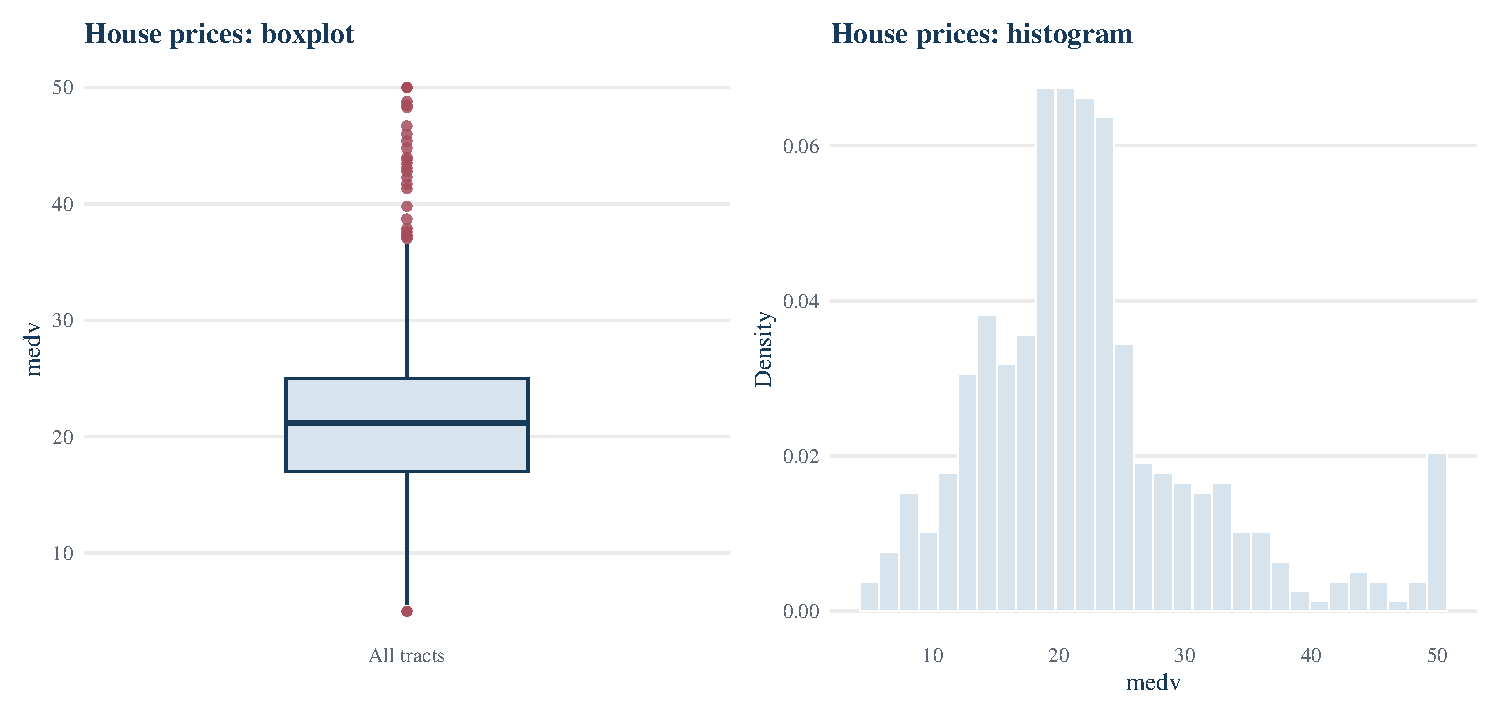
\includegraphics[width=0.86\linewidth]{figure/app_cluster_response_panels-1} 

}

\caption{Full-sample distribution of median house values (\code{medv}, in thousands of US dollars) for the $506$ census tracts in the \code{MASS::Boston} data set. Left panel: boxplot with upper outliers highlighted. Right panel: density-scaled histogram on the same variable.}\label{fig:app_cluster_response_panels}
\end{figure}
\end{Schunk}

\subsection{Model estimation and training cluster summaries}

A bulk only conditional mixture model is applied to the \code{medv}
dataset with three covariates. When \code{type = "weights"},
covariates determine the weights of the mixture while the parameters of the components are common across all covariates. This method is helpful for clustering where the prevalence of latent clusters may differ between neighborhoods.

\begin{Schunk}
\begin{Sinput}
R> .clust_rds <- file.path(manuscript_dir, "saved_fits", "fit_clust.rds")
R> if (file.exists(.clust_rds)) {
+    fit_clust <- readRDS(.clust_rds)
+  } else {
+    fit_clust <- dpmix.cluster(formula = medv ~ ., data = train_dat,
+                               kernel = "normal", type = "weights",
+                               components = 10, mcmc = mcmc_fixed)
+    dir.create(dirname(.clust_rds), showWarnings = FALSE, recursive = TRUE)
+    saveRDS(fit_clust, .clust_rds)
+  }
\end{Sinput}
\end{Schunk}

Since mixture components cannot be identified up to permutation,
clusters in the training data are represented using the posterior
similarity matrix and sample training labels. The posterior similarity
matrix gives the main label-invariant uncertainty summary by
recording posterior clustering probabilities.

\begin{Schunk}
\begin{Sinput}
R> z_train_psm <- predict(fit_clust, type = "psm")
\end{Sinput}
\end{Schunk}
\begin{Schunk}
\begin{Sinput}
R> plot(z_train_psm, type = "summary")
\end{Sinput}
\begin{figure}[!htbp]

{\centering 
\includegraphics[width=0.84\linewidth]{figure/app_cluster_psm_plot-code-1} 

}

\caption{Posterior similarity matrix (PSM) summary for the Boston training sample, returned by \code{plot(predict(fit\_clust, type = "psm"), type = "summary")}. Each cell $(i,\ell)$ encodes the posterior clustering probability $\Pr(z_i=z_\ell\mid\text{data})$, with rows and columns ordered to expose block structure. Darker shading corresponds to higher clustering probability.}\label{fig:app_cluster_psm_plot-code}
\end{figure}
\end{Schunk}

As seen from Figure~\ref{fig:app_cluster_psm_plot-code}, the PSM
reveals clear block structure along the diagonal, implying that the
model can detect multiple sets of tracts whose clustering
probability is relatively high. While there are clear separations,
there are still some uncertainties for those tracts on the edge of
two or more neighboring groups, which reflects reasonable posterior
uncertainty in a non-experimental housing dataset, since features of
neighborhoods tend to change gradually rather than abruptly.

\begin{Schunk}
\begin{Sinput}
R> z_train_lab <- predict(fit_clust, type = "label")
\end{Sinput}
\end{Schunk}
Figure~\ref{fig:app_cluster_overlay} shows the representative training
cluster summary produced by the package \code{plot()} method applied
to the training labels object.

\begin{Schunk}
\begin{Sinput}
R> plot(z_train_lab, type = "summary")
\end{Sinput}
\begin{figure}[!htbp]

{\centering 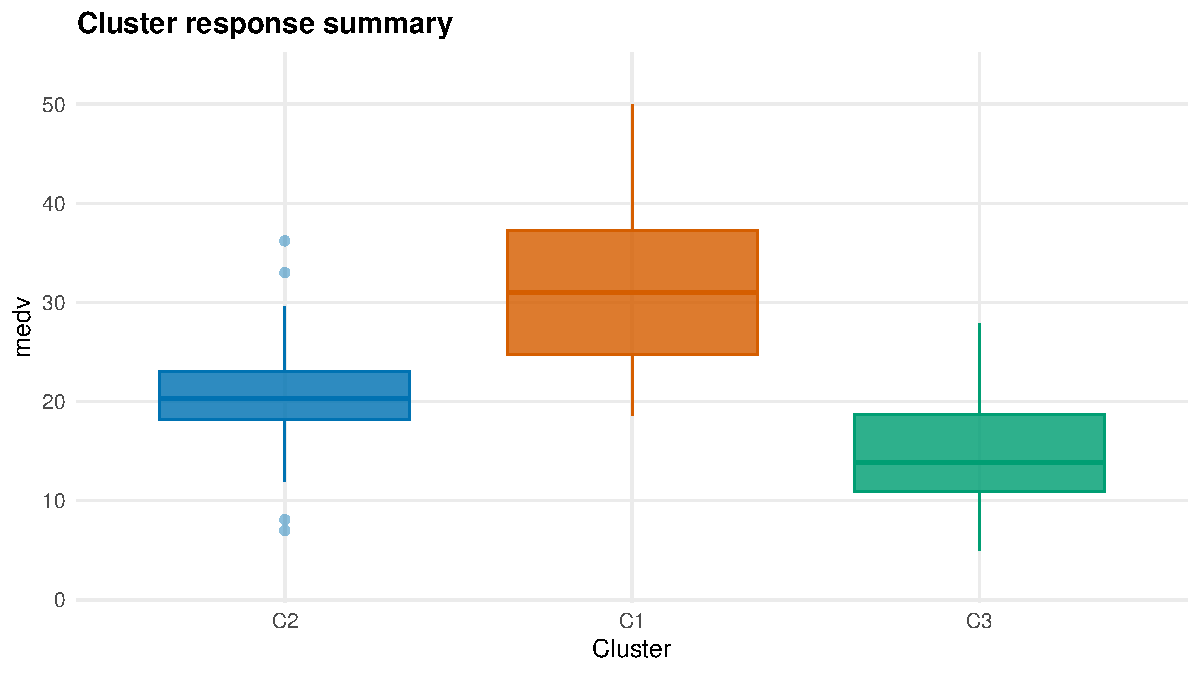
\includegraphics[width=0.84\linewidth]{figure/app_cluster_overlay-1} 

}

\caption[Representative training-cluster summary for the Boston \code{medv} analysis, returned by the \code{plot()} method applied to the labels object from \code{predict(fit\_clust, type = "label")}]{Representative training-cluster summary for the Boston \code{medv} analysis, returned by the \code{plot()} method applied to the labels object from \code{predict(fit\_clust, type = "label")}. Training observations are shown on the response scale and coloured by their assigned cluster in the representative partition.}\label{fig:app_cluster_overlay}
\end{figure}
\end{Schunk}

The representative partition translates the posterior clustering
structure into an interpretable summary on the response scale. The
inferred groups separate tracts primarily by housing-value level, but
they also reflect broader differences in neighborhood composition and
environmental quality. Thus, the clustering output is not merely a
numerical partition induced by the mixture fit; it yields a meaningful
summary of heterogeneity in the Boston housing data.

\subsection{Prediction for new observations}

Cluster assignment for new observations is performed through the same
prediction interface. The output is a label in the space of the
representative training clusters, obtained by aggregating posterior
predictive clustering evidence at the cluster level.

\begin{Schunk}
\begin{Sinput}
R> z_test <- predict(fit_clust, newdata = test_dat, type = "label")
\end{Sinput}
\end{Schunk}

Figure~\ref{fig:app_cluster_test_sizes} displays the distribution of
predicted cluster assignments across the test sample, produced by the
package \code{plot()} method applied to the test labels object.
The printed summary below gives the median response and covariate
profiles for each predicted cluster in the test set, returned by
\code{cluster\_profiles(predict(fit\_clust, newdata = test\_dat, type = "label"))}.

\begin{Schunk}
\begin{Sinput}
R> cluster_profiles(z_test)
\end{Sinput}
\begin{Soutput}
  cluster  n medv_mean  medv_sd  crim_mean   crim_sd   zn_mean
1      C2 46  20.87174 3.133309  0.7925048  1.725793  2.902174
2      C3 30  15.36000 7.796666 13.5420153 18.960580  2.666667
3      C1 26  31.68846 9.695497  1.0496638  1.752975 22.615385
      zn_sd indus_mean indus_sd  chas_mean   chas_sd  nox_mean
1  7.856787  11.349783 6.077225 0.06521739 0.2496374 0.5286957
2 14.605935  18.046333 2.961173 0.03333333 0.1825742 0.6751667
3 27.368708   7.341538 6.405760 0.07692308 0.2717465 0.5259231
      nox_sd  rm_mean     rm_sd age_mean   age_sd dis_mean
1 0.08399335 6.061370 0.3964721 67.79565 28.14555 3.868787
2 0.07969212 6.010900 0.6312801 89.93000 15.24594 2.206400
3 0.11591063 6.884615 1.0538402 58.46923 28.94230 4.199923
    dis_sd  rad_mean   rad_sd tax_mean    tax_sd ptratio_mean
1 1.630337  5.065217 4.291605 319.1087  97.58921     18.43261
2 1.418189 20.600000 7.753086 622.6333 100.56272     19.99000
3 2.196438  8.076923 8.153149 382.9615 150.14885     16.91154
  ptratio_sd black_mean  black_sd lstat_mean lstat_sd
1   1.937244   380.0700  34.36248  11.606522 3.770490
2   1.264461   277.3020 156.42949  19.653000 6.326669
3   2.701307   387.8165  12.37760   6.598462 2.676518
\end{Soutput}
\end{Schunk}
\begin{Schunk}
\begin{Sinput}
R> plot(z_test, type = "sizes")
\end{Sinput}
\begin{figure}[!htbp]

{\centering 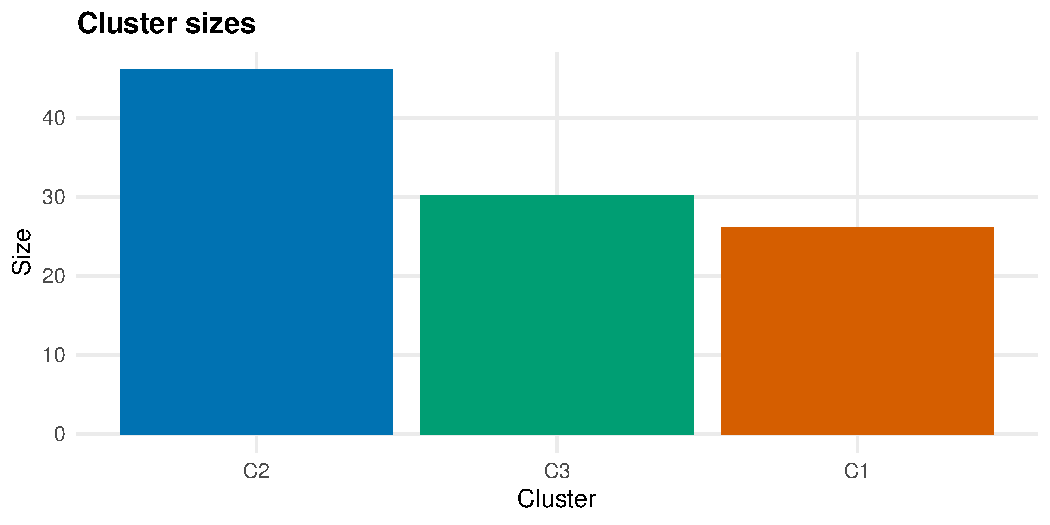
\includegraphics[width=0.80\linewidth]{figure/app_cluster_test_sizes-1} 

}

\caption{Bar plot of predicted cluster assignments for the held-out Boston test sample (the $20\%$ of \code{medv} observations excluded from training), returned by \code{plot(predict(fit\_clust, newdata = test\_dat, type = "label"), type = "sizes")}. Each bar corresponds to one representative training cluster from Figure~\ref{fig:app_cluster_overlay}; bar heights give the number of test tracts assigned to that cluster.}\label{fig:app_cluster_test_sizes}
\end{figure}
\end{Schunk}

The obtained profiles for the clusters correspond to our expectations concerning the representative partition. Cluster C1 includes tracts with higher average house values (\code{medv}), more rooms (\code{rm}), greater residential zoning (\code{zn}), and lower pollution (\code{nox}). On the contrary, cluster C3 represents the poorer area with fewer rooms (\code{rm}), low house value (\code{medv}), high rate of crime (\code{crim}) and industrialization (\code{indus}), and the highest level of average pollution (\code{nox}). Cluster C2 represents an area in between. For test data, clusters characterized by larger average house prices (\code{medv}) have fewer neighborhood disadvantages such as lower crime per capita (\code{crim}), more spacious houses (\code{rm}), and less pollution (\code{nox}); poorer clusters represent the opposite pattern.

The presented case study demonstrates the usage of a representative partition and its cluster description as well as how we assign posterior predictive membership probabilities for a new observation. The use of representative clusters makes the connection between partition uncertainty and distribution of the response given covariates clearer.

\section{Data analysis~II: causal inference}
\label{sec:app-causal}

This section describes the estimands from the two-arm spliced density regression. In contrast to the partition estimation of Section~\ref{sec:app-clustering}, the focus here is on mean and quantile differences for both unconditional and conditional causal estimands.

\subsection{Data and estimands}

To estimate unconditional and conditional causal estimands using the proposed approach, the \code{lalonde} dataset from the \pkg{MatchIt} \proglang{R} package is used for benchmarking. The outcome is the 1978 annual income level measured by \code{re78} (\$), and the treatment indicator corresponds to program participation (variable \code{treat}). Covariates include age, years of schooling, race, marriage status, college degree status, and prior earnings \code{re74} and \code{re75}. Earnings typically exhibit considerable skewness, concentrate near zero, and have a pronounced upper tail, motivating the use of quantile and tail summaries rather than the mean alone.

The six estimands in Table~\ref{tab:causal-estimands-main} are computed following Section~\ref{subsec:causal}. Standardized estimands (ATE, QTE) are averaged across the empirical distribution of \(\{\boldsymbol{x}_i\}_{i=1}^n\), while conditional estimands (CATE, CQTE) are evaluated at selected covariate profiles.

The data are first loaded and the design matrix constructed.

\begin{Schunk}
\begin{Sinput}
R> data("lalonde", package = "MatchIt")
R> app_lalonde_covars <- within(lalonde, {
+      race <- factor(race, levels = c("white", "black", "hispan"))
+      married <- factor(married, levels = c(0, 1), labels = c("no", "yes"))
+      nodegree <- factor(nodegree, levels = c(0, 1), labels = c("no", "yes"))
+  })
R> app_lalonde_scale_vars <- c("age", "educ", "re74", "re75")
R> app_lalonde_scale_center <- vapply(
+      app_lalonde_scale_vars,
+      function(v) mean(app_lalonde_covars[[v]], na.rm = TRUE),
+      numeric(1)
+  )
R> app_lalonde_scale_scale <- vapply(
+      app_lalonde_scale_vars,
+      function(v) stats::sd(app_lalonde_covars[[v]], na.rm = TRUE),
+      numeric(1)
+  )
R> for (v in app_lalonde_scale_vars) {
+      app_lalonde_covars[[paste0(v, "_z")]] <-
+          (app_lalonde_covars[[v]] - app_lalonde_scale_center[[v]]) /
+          app_lalonde_scale_scale[[v]]
+  }
R> app_lalonde_x_formula <- ~age_z + educ_z + race + married +
+      nodegree + re74_z + re75_z
R> app_lalonde_y <- (app_lalonde_covars$re78 + 0.5)/1000
R> app_lalonde_A <- as.integer(app_lalonde_covars$treat)
R> app_lalonde_taus <- c(0.25, 0.5, 0.75, 0.9, 0.95)
R> app_lalonde_X <- stats::model.matrix(
+      app_lalonde_x_formula,
+      data = app_lalonde_covars)[, -1, drop = FALSE]
\end{Sinput}
\end{Schunk}

Figure~\ref{fig:app_lalonde_response_panels} provides full-sample
descriptive views of observed 1978 earnings (\code{re78}) by treatment
assignment. Both groups exhibit substantial mass near zero together
with pronounced right-skewness, and the arm-specific distributions
differ in ways that are not well summarized by a simple location shift.
These features motivate modeling the full treatment-specific outcome
distributions directly rather than relying solely on average effects.

\begin{Schunk}
\begin{figure}[!htbp]

{\centering 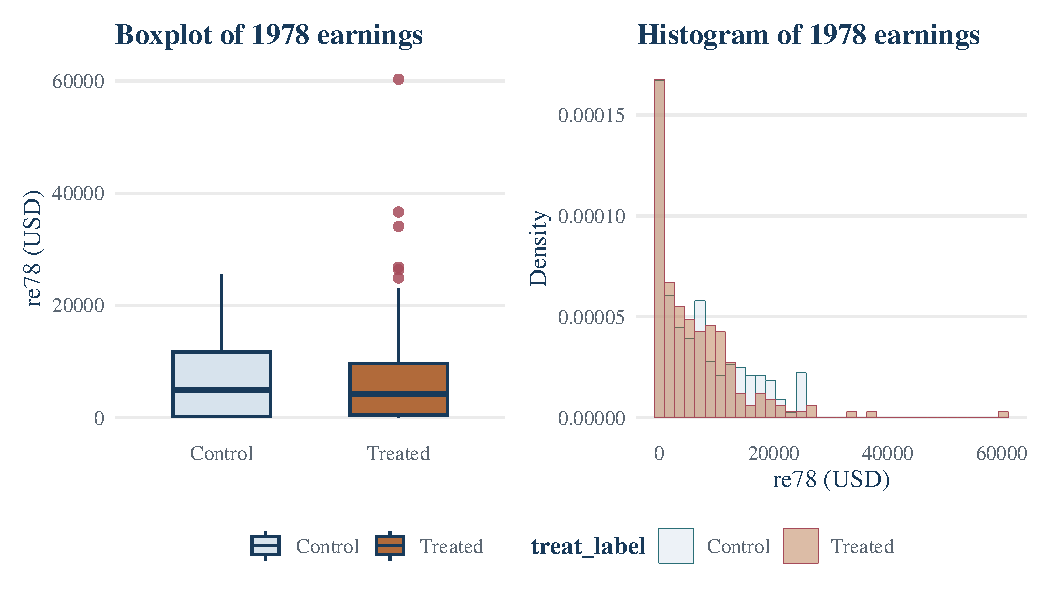
\includegraphics[width=0.88\linewidth]{figure/app_lalonde_response_panels-1} 

}

\caption{Full-sample distribution of 1978 annual earnings (\code{re78}, in US dollars) from the \code{MatchIt::lalonde} data set, stratified by treatment arm. Left panel: arm-specific boxplots with upper outliers highlighted. Right panel: overlaid density-scaled histograms for the control and treated arms.}\label{fig:app_lalonde_response_panels}
\end{figure}
\end{Schunk}

\subsection{Model and fit}

Arm-specific conditional outcome distributions
$F_a(\cdot\mid \boldsymbol{x})$ are modeled via the spliced bulk--tail
construction described in Section~\ref{subsec:splice}:
\begin{equation*}
\begin{aligned}
f_a(y\mid \boldsymbol{x})
={}&
\sum_j w_{aj}(\boldsymbol{x})\, k(y\mid \Theta_{aj})\,\mathbf{1}(y\le u)\\
&+
\{1-F_a(u\mid \boldsymbol{x})\}\, g(y\mid u,\sigma_a,\xi_a)\,\mathbf{1}(y>u).
\end{aligned}
\end{equation*}
The bulk kernel $k(\cdot)$ represents a Dirichlet process mixture
regression with a Chinese restaurant process backbone, while the tail
density $g(\cdot)$ follows the GPD distribution with positive scale
$\sigma_a>0$ and tail index $\xi_a$. In our model, the GPD tail index
$\xi_a$ regulates tail heaviness (e.g., if $\xi_a>0$, it indicates a
heavier tail). Our model mitigates poor finite-sample precision for extreme
quantiles through nonparametric bulk and EVT-consistent tail modeling.

Here, a two-sample mixture is fitted with the gamma bulk kernel and the
same MCMC configuration throughout. The aim is not to draw definitive
conclusions but to demonstrate how the package produces standardized and
conditional earnings contrasts under the spliced DPM-GPD framework.

\begin{Schunk}
\begin{Sinput}
R> fit <- dpmgpd.causal(y = app_lalonde_y, X = app_lalonde_X,
+                       treat = app_lalonde_A,  backend = "crp",
+                       kernel = "gamma", components = 10,  mcmc = mcmc_fixed)
\end{Sinput}
\end{Schunk}



\subsection{Posterior summaries}

The fitted causal object defines two arm-specific outcome distributions
from which all reported summaries are derived. The framework is therefore
not limited to a single regression coefficient or scalar contrast; mean,
quantile, and tail-sensitive causal estimands are all coherent functionals
of the same fitted posterior distribution.

\subsection{Standardized estimands: ATE and QTE}

The overall treatment effect is summarized with ATE and QTE.

\begin{Schunk}
\begin{Sinput}
R> ate_fit <- ate(fit, interval = "hpd", level = 0.95)
R> summary(ate_fit)
\end{Sinput}
\begin{Soutput}
ATE Summary
================================================== 
Prediction points: 1
Conditional: NO | PS used: YES
Interval: hpd

Model specification:
  Backend (trt/con): crp / crp
  Kernel (trt/con): gamma / gamma
  GPD tail (trt/con): YES / YES

ATE estimates:
 estimate  lower upper
   -2.543 -5.341 0.396
\end{Soutput}
\end{Schunk}

The posterior ATE estimate is negative on the scaled earnings scale,
but the corresponding interval includes zero. Thus, after averaging
over the empirical covariate distribution, the analysis does not
provide strong evidence of a uniform overall mean effect of the
training program.

\begin{Schunk}
\begin{Sinput}
R> qte_fit <- qte(fit, probs = c(0.25, 0.5, 0.75),
+                interval = "credible")
\end{Sinput}
\end{Schunk}

Figure~\ref{fig:qte_plot} displays two standardized QTE views side by
side from the causal model: the estimated QTE profile across the
evaluated quantiles and the treated-versus-control quantile summaries
with uncertainty intervals.

\begin{Schunk}
\begin{Sinput}
R> qte_effect_plot <- plot(qte_fit, type = "effect")
R> qte_arms_plot <- plot(qte_fit, type = "arms")
R> qte_effect_plot + qte_arms_plot + plot_layout(ncol = 2)
\end{Sinput}
\begin{figure}[!htbp]

{\centering 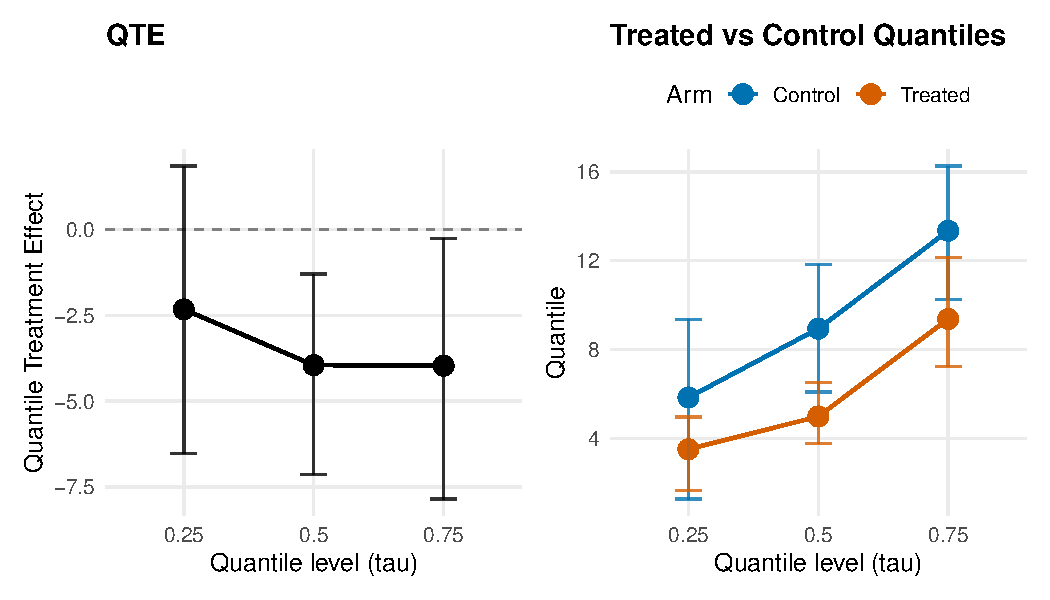
\includegraphics[width=0.88\linewidth]{figure/qte_plot-1} 

}

\caption{Standardized quantile treatment effect (QTE) summaries for Lalonde 1978 earnings, returned by \code{qte(fit, probs = c(0.25, 0.50, 0.75), interval = "credible")}. Left panel: effect curve $Q_1^{\mathrm{m}}(\tau)-Q_0^{\mathrm{m}}(\tau)$ versus $\tau$ with pointwise $95\%$ credible band. Right panel: standardized treated and control quantile curves $Q_1^{\mathrm{m}}(\tau)$ and $Q_0^{\mathrm{m}}(\tau)$ on the original earnings scale, with pointwise credible bands.}\label{fig:qte_plot}
\end{figure}
\end{Schunk}

Estimates of QTEs are all negative for the quantiles analyzed. However, the confidence interval for the median QTE and the for the 3rd quartile do not contain zero, indicating that the training program have a negative impact on high earners.


\subsection{Conditional estimands for representative profiles}

To characterize heterogeneity in the treatment effect, conditional estimands are computed at four representative covariate profiles spanning the observed covariate range. Profile values are expressed on the original data scale, using empirical quantiles for continuous variables and observed levels for categorical variables. Continuous predictors are standardized using training-set means and standard deviations before being passed to the model.



\begin{table}
\centering
\caption{\label{tab:xnew-results}Representative Lalonde participant profiles used as new-data inputs for the conditional causal contrasts reported in Figure~\ref{fig:cate_plot} and in the printed CQTE summary below. Columns (Profile~1--Profile~4) give the covariate values for one synthetic individual on the original data scale: \code{age} (years), \code{educ} (years of schooling), \code{race}, \code{married}, \code{nodegree}, and prior annual earnings \code{re74} and \code{re75} (US dollars).}
\centering
\resizebox{\ifdim\width>\linewidth\linewidth\else\width\fi}{!}{
\fontsize{8}{10}\selectfont
\begin{tabular}[t]{lllll}
\toprule
  & Profile 1 & Profile 2 & Profile 3 & Profile 4\\
\midrule
age & 20.0000 & 25.0000 & 32.0000 & 43.0000\\
educ & 9.0000 & 11.0000 & 12.0000 & 13.0000\\
race & black & hispan & white & black\\
married & no & no & yes & yes\\
nodegree & yes & no & no & yes\\
\addlinespace
re74 & 0.0000 & 47.4143 & 2705.7476 & 9383.2356\\
re75 & 0.0000 & 16.4710 & 1389.6486 & 4201.8870\\
\bottomrule
\end{tabular}}
\end{table}



\begin{Schunk}
\begin{Sinput}
R> cate_fit <- cate(fit, newdata = xnew, interval = "hpd")
R> summary(cate_fit)
\end{Sinput}
\begin{Soutput}
CATE Summary
================================================== 
Prediction points: 4
Conditional: YES | PS used: YES
Interval: hpd

Model specification:
  Backend (trt/con): crp / crp
  Kernel (trt/con): gamma / gamma
  GPD tail (trt/con): YES / YES

CATE estimates:
   profile estimate   lower upper
 Profile 1   -1.978  -5.481 1.448
 Profile 2   -2.685  -7.837 1.612
 Profile 3   -1.744  -7.203 3.256
 Profile 4   -7.725 -31.332 15.31
\end{Soutput}
\end{Schunk}

Figure~\ref{fig:cate_plot} shows the  CATE summaries across
the four representative profiles.
\begin{Schunk}
\begin{figure}[!htbp]

{\centering 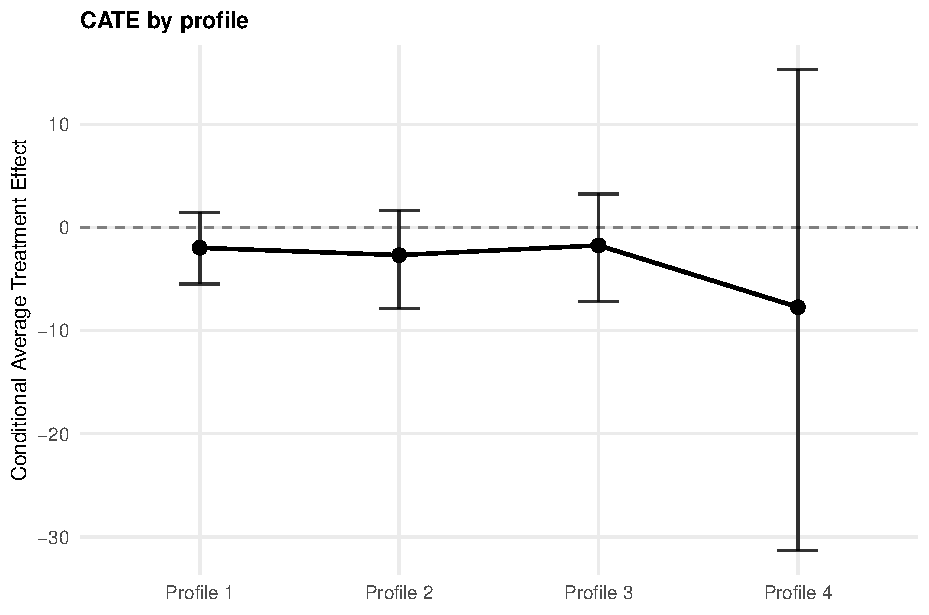
\includegraphics[width=0.76\linewidth]{figure/cate_plot-1} 

}

\caption{Profile-specific conditional average treatment effects for Lalonde 1978 earnings at the four representative covariate profiles (Profile~1--Profile~4) of Table~\ref{tab:xnew-results}, returned by \code{cate(fit, newdata = xnew, interval = "hpd")}. Points denote posterior estimates of $\mathrm{CATE}(x)=\mu_1(x)-\mu_0(x)$ and vertical bars give $95\%$ HPD intervals.}\label{fig:cate_plot}
\end{figure}
\end{Schunk}


None of the four profiles show a statistically significant  CATE, as all 95\% HPD intervals include zero. However, the point estimates suggest that the program may have a negative effect on earnings for Profiles~4, while the effects for Profiles~1, 2 and~4 are closer to zero.
\begin{Schunk}
\begin{Sinput}
R> cqte_fit <- cqte(fit, probs = c(0.25, 0.5, 0.75, 0.9, 0.95),
+                   newdata = xnew, interval = "credible")
R> summary(cqte_fit)$effect_table
\end{Sinput}
\begin{Soutput}
     profile  tau      estimate       lower      upper
1  Profile 1 0.25  -2.521841198   -7.744296  4.0271372
2  Profile 1 0.50  -3.717253897   -7.385001 -0.6244419
3  Profile 1 0.75  -3.036742586   -7.347654  1.4575352
4  Profile 1 0.90  -1.616077528   -7.876948  5.9154540
5  Profile 1 0.95  -0.002597363   -8.645220 10.5596639
6  Profile 2 0.25  -1.388753348   -8.374172  3.5607329
7  Profile 2 0.50  -4.461346476   -9.850380 -0.1311481
8  Profile 2 0.75  -4.406719223  -10.769044  0.5638009
9  Profile 2 0.90  -3.966523104  -11.325236  3.6031938
10 Profile 2 0.95  -3.546162922  -13.181625  6.9877301
11 Profile 3 0.25  -1.400116612   -6.699770  2.7939363
12 Profile 3 0.50  -1.800035981   -7.721600  3.5216058
13 Profile 3 0.75  -2.604699710   -8.484734  4.2098620
14 Profile 3 0.90  -2.871274028   -8.828207  4.2015030
15 Profile 3 0.95  -2.528672343  -10.414719  8.3735820
16 Profile 4 0.25  -2.553434640   -9.052905  4.3991099
17 Profile 4 0.50  -5.901260763  -17.654505  6.3991686
18 Profile 4 0.75 -11.486181749  -45.838709 20.1632763
19 Profile 4 0.90 -19.094601788  -86.637680 42.1730175
20 Profile 4 0.95 -24.260813769 -119.477696 64.8149038
\end{Soutput}
\end{Schunk}



The CQTE estimates reveal heterogeneity across all covariate profiles and quantile levels. At low and median quantile levels, the estimated program effect is negative or close to zero, with the median CQTE significantly below zero for Profiles~1 and~2. Uncertainty increases sharply at the upper quantiles, especially for Profile~4, because upper-quantile contrasts rely on fewer observations and are more sensitive to the spliced tail. Overall, the CQTE table provides no clear evidence of positive program effects: upper-tail intervals sometimes extend into positive values, but the corresponding point estimates remain negative.

\subsection{Results and interpretation}

Two questions bear on the interpretation: the overall program effect on earnings, and heterogeneity of effects across participant profiles. The first yields no statistically compelling evidence: the average treatment effect is close to zero and the estimated QTE are negative at lower and mid-quantiles. The second indicates heterogeneity in magnitude and uncertainty across profiles, but not a clear reversal in sign: CQTE point estimates remain nonpositive across the reported quantiles, while upper-tail intervals widen substantially for some profiles.

This analysis underscores the value of quantile-based methods for heavy-tailed outcomes. A mean-only analysis provides little evidence of a program effect; the QTE, by contrast, reveals heterogeneity in the treatment effect across the outcome distribution.

\section{Discussion}
\label{sec:discussion}

\pkg{CausalMixGPD} combines flexible bulk density estimation,
optional EVT-based tail extrapolation, predictor-dependent clustering,
and quantile- and density-level causal inference within one package.
The same fitted model supports posterior summaries for densities,
survival summaries, analytical means (when they exist), restricted means,
quantiles, and treatment contrasts. This is useful in settings where
heavy tails and density-level effects are both of concern.

The package is considerably broader than the examples
emphasized in this article.  Users may work with bulk-only or spliced
models, multiple kernel families on the real line or on positive
support, stick-breaking or CRP backends, and clustering or causal
wrappers built upon the same predictive machinery.  This shared
infrastructure lets users move from exploratory subgroup analysis to
tail-focused prediction and causal reporting without changing the
underlying modeling language.

Several practical limitations warrant acknowledgment.  First,
computation can be demanding.  Mixture models with covariate
dependence, optional tail components, and arm-specific causal fits are
inherently MCMC-intensive, and costs escalate further with sensitivity
analyses, longer chains, or richer predictor sets.

Second, model tuning requires attention.  A spliced analysis inherits
specification choices from both the DPM and peaks-over-threshold
components, including kernel family, truncation level, threshold
specification, and the number of exceedances available for tail
learning.  When overlap is weak or exceedances are sparse, posterior
uncertainty can be misleading; for clustering, the posterior
similarity matrix is often more informative than any single partition
summary.

Third, the current scope is circumscribed.  The causal implementation
is restricted to binary treatments and continuous outcomes under
standard consistency, ignorability, and overlap assumptions.
Propensity-score augmentation can improve covariate adjustment in
observational studies, but it is not a substitute for careful study
design, overlap diagnostics, or sensitivity analysis for unmeasured
confounding.

Finally, this article treats \pkg{CausalMixGPD} as a software
contribution and describes the implemented modeling workflow
self-containedly.  Formal methodological development beyond the
software and examples presented here should be evaluated separately
from the package interface, documentation, and replication material.

\section{Software Availability}
\label{sec:software}

Version 0.8.0 of the \pkg{CausalMixGPD} R package is the version used
for this article. The package is licensed under GPL-3 and is available
from CRAN.
The development version is available from the GitHub repository
\url{https://github.com/arnabaich96/CausalMixGPD}.

\section*{Acknowledgements}
The author thanks Dr. Indrabati Bhattacharya for her insightful comments to this work.

\section*{Funding}
This research did not receive any specific grant from funding agencies in the
public, commercial, or not-for-profit sectors.

\section*{Declaration of competing interest}
The author declares that he has no known competing financial interests or
personal relationships that could have appeared to influence the work reported
in this paper.

\section*{Declaration of generative AI}
During the preparation of this work the author used Claude Opus 4.8 (Anthropic)
and ChatGPT vesion 5.5 (OpenAI) in order to improve the language and readability of the
manuscript. After using these tools, the author reviewed and edited the content
as needed and takes full responsibility for the content of the published article.

\makeatletter
\IfFileExists{manuscript/CausalMixGPD_JSS_refs.bib}{%
  \bibliographystyle{manuscript/elsarticle/elsarticle-harv}%
  \bibliography{manuscript/CausalMixGPD_JSS_refs}%
}{%
  \bibliographystyle{elsarticle/elsarticle-harv}%
  \bibliography{CausalMixGPD_JSS_refs}%
}
\makeatother
\clearpage
\appendix
\section{Customization of package and additional features}
\label{sec:appendix-features}

This appendix details the customizable features of \pkg{CausalMixGPD}. It covers argument-level customization for model fitting, posterior manipulation, and workflow-specific extensions.

\subsection{Model fitting options and prior specifications}
\label{subsec:app-modeling}

Besides the customizable features illustrated in Sections \ref{subsec:gpd}, \ref{subsec:dpm}, \ref{subsec:causal}, and \ref{subsec:overview-model}, this section lists arguments that allow kernel choice, latent structure, and prior customization alternative to default choices.

\begin{itemize}
\item \textbf{Kernel families and support}: the argument \code{kernel} selects one of seven kernel families on either the positive line or the real line. Positive-support options include \code{"gamma"} and \code{"lognormal"}. They also include \code{"invgauss"} and \code{"amoroso"}. Real-line options are \code{"normal"}, \code{"laplace"}, and \code{"cauchy"}. For causal models, \code{kernel} can be a single string or a length-two vector specifying different DPM kernels for the two arms. The choice of kernel should match the support of the outcome variable.

\item \textbf{Backend type and truncation rule}: the argument \code{backend} determines the structure of the mixing coefficients. The value \code{sb} stands for the stick-breaking scheme while \code{crp} denotes the Chinese Restaurant Process latent allocation scheme. For causal models, \code{backend} can be either a single string or a length-two vector specifying different latent allocation schemes for the two arms. The argument \code{components} sets the maximum number of mixture components (defaulting to the sample size). The argument \code{epsilon} specifies a truncation threshold below which components are dropped and the smallest weight is readjusted. Both arguments can be customized separately for each causal arm.

\item \textbf{Parameter specification and prior setting}: the argument \code{param_specs} is a named list giving the parameters of the kernel or tail distribution. Each kernel/tail parameter supports three modes: \code{"fixed"}, \code{"dist"}, and \code{"link"}. With \code{"dist"}, the prior can be chosen as any distribution compatible with the parameter and supported by \pkg{nimble}, with hyperparameters specified in the default registry. With \code{"link"}, the kernel/tail parameter is related to the covariates through a linear regression using one of five link functions (\code{"identity"}, \code{"exp"}, \code{"log"}, \code{"softplus"}, or \code{"power"}); the link power is adjusted via \code{link_power} when the last option is selected. With \code{"fixed"}, the parameter is fixed to the constant value specified in \code{param_specs}. For causal models, \code{param_specs} can be either a single named list or a length-two list specifying different parameter specifications for the two arms.
\end{itemize}

\subsection{Fitting, prediction, and posterior output}
\label{subsec:app-fitting}

This section gathers the arguments used after a model class has been chosen: sampler configuration, monitoring, and fitting interfaces.

\begin{itemize}
\item \textbf{MCMC configuration}: \code{mcmc} controls \code{niter}, \code{nburnin}, \code{thin}, \code{nchains}, and \code{seed}; causal models split this into \code{mcmc\_outcome} and \code{mcmc\_ps}. Runtime controls include \code{show\_progress}, \code{quiet}, \code{parallel\_chains} with \code{workers}, \code{parallel\_arms} for arm-wise causal fitting, and \code{timing}. CRP-based backends additionally use \code{z\_update\_every} to tune the frequency of global label updates.
\item \textbf{Monitoring and fitting interfaces}: \code{monitor = "core"} retains the main structural parameters, whereas \code{"full"} retains all nodes. \code{monitor\_latent = TRUE} stores allocation labels $z_1,\ldots,z_n$, and \code{monitor\_v = TRUE} stores stick-breaking fractions for SB models. Models can be supplied through a formula interface (\code{formula}, \code{data}) or directly through \code{y} and \code{X}; causal fits additionally use \code{treat}.

\end{itemize}

\subsection{Workflow-specific extensions}
\label{subsec:app-workflows}

This section records controls specific to the clustering and causal workflows in Sections~\ref{subsec:cluster_extension}, \ref{subsec:overview-causal}, \ref{sec:app-clustering}, and \ref{sec:app-causal}. Representative outputs appear in Figures~\ref{fig:app_cluster_overlay}, \ref{fig:app_cluster_test_sizes}, \ref{fig:qte_plot}, and \ref{fig:cate_plot}.

\begin{itemize}
\item \textbf{Propensity score customization}: observational causal fits can estimate propensity scores with \code{PS = "logit"}, \code{"probit"}, \code{"naive"}, or \code{FALSE}. The estimated score is appended to the outcome model on either the logit scale, \code{ps\_scale = "logit"}, or the probability scale, \code{"prob"}. Posterior summaries use \code{ps\_summary = "mean"} or \code{"median"}. Numerical stability is controlled through \code{ps\_clamp}, shrinkage through \code{ps\_prior}, and the two-stage fitting scheme through separate \code{mcmc\_ps} and \code{mcmc\_outcome} lists.
\item \textbf{Clustering dependence mode}: clustering fits accept \code{type = "weights"}, \code{"param"}, or \code{"both"} to place predictor dependence in the mixture weights, kernel parameters, or both. The \code{newdata} argument controls whether label assignment is restricted to training observations or extended to additional covariate profiles.

\end{itemize}

\subsection{Utilities and computing support}

The last appendix section includes computing and data resources that
accompany the main modeling process.

\begin{itemize}
\item \textbf{Simulators and bundled datasets}: the package includes reproducible benchmark generators for bulk, tail, and causal analyses. Random-number seeds are supplied by the \code{seed} argument. The package also bundles twelve datasets spanning unconditional, conditional, and causal settings on positive and real-line supports, with and without tail components.
\item \textbf{Computational considerations}: large-scale analyses can use \code{parallel\_chains} with \code{workers}, \code{parallel\_arms} for causal fits, \code{chunk\_size} for prediction in parallel chunks, and \code{ndraws\_pred} for sampling from posterior predictive parameter distributions. The \code{show\_progress} and \code{quiet} arguments control progress reporting and compiler verbosity, while \code{timing = TRUE} records runtime summaries.
\end{itemize}

\end{document}

